\chapter{Vortex connections across topological interfaces}\label{chap: spin-2}
\section{To do}
\begin{itemize}
    \item 
\end{itemize}


Topological interfaces may form at the phase boundary between topologically
distinct phases that are described by different order parameters.
In such an interface, the phases can exist in a coherent and order medium, in
which the different symmetries connect smoothly across the boundary.
Such interfaces arise in many areas of physics, such as the context of domain
walls in the early universe~\cite{Zeldovich1975,Kibble1976,Kibble1980}, where
they may form the termination points of cosmic strings~\cite{Vilenkin1985},
brane models in superstring theory~\cite{Dvali1999,Sarangi2002,Gudnason2015},
the \(A\)--\(B\) phase boundary in superfluid liquid \(^3\)He~\cite{
    Osheroff1977,Yip1986,Salomaa1987,Finne2006,Bradley2007,Volovik2009}, via
atomic Bose-Einstein condensates (BECs)~\cite{Takeuchi2006,Kasamatsu2010,
    Borgh2012,Borgh2013, Borgh2014,Kaneda2014}, and even quantum
chromodynamics~\cite{Alford2001,Cipriani2012,Eto2014}.
The differing order parameter symmetry on each side of the interface implies
that families of vastly different defects and textures may exist, and therefore
cannot cross the interface unchanged.
Instead, the defect must either terminate at the boundary, or continuously
and non-trivially connect to an object representing a different topology on the
other side of the interface.

Since Spinor BECs carry a rich phase diagram which support a wide family of
topological defects exhibiting different order parameter symmetries, they become
an ideal test bed for investigating interface physics~\cite{Borgh2012,Borgh2013,
    Borgh2014}.
Such defects include singular vortices carrying both integer~\cite{Yip1999,
    Isoshima2002,Mizushima2002a,Zhou2003,Sadler2006,Semenoff2007,Kobayashi2009,
    Lovegrove2012,Lovegrove2016,Borgh2016a,Weiss2019,Xiao2021,Xiao2022} and
fractional~\cite{Leonhardt2000,Ji2008,Seo2015,Semenoff2007,Lovegrove2012,
    Lovegrove2016,Borgh2016a,Borgh2017,Xiao2021,Xiao2022} charges, as well as
non-singular vortices (2D Skyrmions)~\cite{Ohmi1998, Ho1998, Mizushima2002,
    Martikainen2002, Leanhardt2003, Mizushima2004, Choi2012, Choi2012a,
    Lovegrove2014,Weiss2019}, wall-vortex complexes~\cite{Kang2019,
    Takeuchi2021}, and monopoles~\cite{Stoof2001,
    Savage2003,Ruostekoski2003,Pietila2009,Ray2014,Ray2015,Ollikainen2017,
    Mithun2022}.
In addition, non-Abelian defects, whose charges depend on other defects within
the system, may arise when the medium on either or both sides of the interface
exhibits point-group order parameter symmetry~\cite{Xiao2022}.

In this chapter, we both analytically and numerically investigate the physics
of topological defects when connected across topological interfaces in spin-2
Bose-Einstein condensates.
We demonstrate that a particularly rich phenomenology of topological defects
at the coherent
interface between regions of different broken symmetries can be realised in
spin-2 Bose-Einstein condensates.
In particular, we propose that an interface between uniaxial and biaxial nematic
phases exhibiting continuous and discrete order-parameter symmetry,
respectively, can be realised using existing experimental techniques.
We construct spinor wave functions that represent topological defects connecting
across the interface.
By numerical energy relaxation as well as simulations of dynamics, we
characterise the emergence of non-trivial defect core structures.
We further demonstrate the emergence of composite vortex-core structures and
continuous connection of fractional vortices representing non-Abelian charges in
interfaces involving the cyclic and ferromagnetic phases, which could be
realised through manipulation of the inter-atomic interactions.
Our results suggest the spin-2 Bose-Einstein condensates as experimentally
accessible test beds for interface physics with all combinations of continuous
and discrete symmetries, as well as phases supporting non-Abelian defects.

\section{Interface crossing solutions in a spin-2 BEC}
\textcolor{red}{Move this paragraph later on, focus on interfaces in the BEC
itself first.}
In a continuous spinor superfluid, it is possible for distinct phases with
varying order parameter symmetry to coexist.
This situation can arise, for example, due to energy relaxation in vortex core
structures~\cite{Ruostekoski2003,Lovegrove2012,Lovegrove2016,Borgh2016,
    Borgh2016a, Weiss2019,Xiao2021,Xiao2022}.
In a spin-2 BEC, the three contributions to the interaction energy each give
rise to a healing length, which describe, respectively, the distance over which
perturbations of the superfluid density, condensate spin, and singlet duo
amplitude heal to the bulk value:
\begin{equation}
    \xi_d=\ell \sqrt{\frac{\hbar\omega}{2nc_0}},
    \enskip \xi_F=\ell \sqrt{\frac{\hbar\omega}{2n|c_1|}},
    \enskip \xi_a=\ell \sqrt{\frac{\hbar\omega}{2n|c_2|}},
    \label{eq: spin-2-healing-lengths}
\end{equation}
where \(\ell = {(\hbar/M\omega)}^{1/2}\) is the harmonic oscillator length.
Typically, \(\xi_F,\xi_a > \xi_d\), allowing the core of singular vortices
to reduce its energy by expanding and filling with a different superfluid
phase~\cite{Ruostekoski2003}.
The condensate wave function then smoothly interpolates between the coexisting
phases in the bulk superfluid and the defect core, establishing a topological
interface between them.

A spinor BEC may be engineered such that separate regions of the condensate
have distinct ground state phases, e.g., nematic or cyclic, and hence have
different order parameter symmetries, creating a topological interface within
the condensate itself.
This can be achieved through variation of parameters in the Hamiltonian (see
\textcolor{red}{Link to spin-2 Hamiltonian}), such as the linear and quadratic
Zeeman shifts, which locally stabilise the different regions.
If the parameter fluctuation is sufficiently acute, then the wave function will
interpolate between the bulk phases across a distance given by an appropriate
healing length.
In addition, as proposed for the spin-1 system~\cite{Borgh2014}, linear \(p\)
and quadratic \(q\) Zeeman shifts form the basis for engineering interpolating
solutions that model the topological interface.
Such steady-state solutions are found from the mean-field Hamiltonian density
functional in Eq.~(\textcolor{red}{No full spin-2 Hamiltonian in paper, either
    put here or back in Chapter 2}) for a uniform system in the presence of an
external magnetic field using the relation \(\delta \mathcal{H}
/ \delta \zeta_m^*=0\)~\cite{Kawaguchi2012}:
\begin{equation}\label{eq: spin-2-GPEs-time-reversal}
    \left[-p \hat{F}_z + q \hat{F}^2_z + c_0n \, \zeta^\dagger \zeta
        + c_1n \, \langle\hat{\vb{F}}\rangle\cdot\hat{\vb{F}}
        + \frac{c_2n}{5}{(\hat{\mathcal{T}}\zeta)}^\dagger \,
        \zeta\hat{\mathcal{T}} -\mu \right] \zeta = 0,
\end{equation}
where \(\mu \) is the chemical potential and \(\hat{\mathcal{T}}\) is a
time-reversal operator defined as \({(\hat{\mathcal{T}}\zeta)}_m =
{(-1)}^m\zeta_{-m}^*\).
Eq.~\eqref{eq: spin-2-GPEs-time-reversal} presents a non-linear system of
equations that can be solved for the unknown
\(\zeta_m\)~\cite{Ciobanu2000,Kawaguchi2012}.

Using the constructed interpolating stationary states, defect states for a given
spin-2 phase can, in principle, be constructed from
the representative spinor by defining an appropriate azimuthal phase winding,
\(\chi_m \), in each component, i.e., \(\text{Arg}(\zeta_m) =\chi_m =
k_m\varphi \), where \(k_m\) is an integer and \(\varphi \) is the azimuthal
angle around the vortex core.
In addition, we also create a unitary framework which is applicable for
constructing other types of defect states across topological interfaces in a
spin-2 BEC, such as monopoles or textures.
A given defect state can be constructed from the uniform state by applying a
global phase winding, \(\tau \), coupled with a spin rotation defined by three
Euler angles \((\alpha, \beta, \gamma)\) as in
Eq.~\eqref{eq: spin-2-rotation-matrix}.
When the same transformation is supported by two phases, A and B, of a spin-2
condensate, a general defect connection across an interface between the two
phases is given as
\begin{align}\label{eq: general-defect-interface}
    \zeta = e^{i\tau}\,\hat{U}(\alpha, \beta, \gamma)\,\zeta^\text{A-B}.
\end{align}
Through the subsequent sections we provide various steady-state solutions that
interpolate between the different phases of a spin-2 BEC.\@
Using these solutions, we then construct interesting defect states that connect
across the topological interface.
Detailed derivations of each interpolating solution used in the subsequent
sections can be found in Appendix~\ref{appendix: stationary}.

\subsection{Uniaxial nematic to biaxial nematic}\label{subsec: UN-BN-defects}
We first focus on a family of solutions interpolating between the UN and BN
phases (see Sec~\ref{sec: ground-states-spin-2} for details on these ground
states).
Such an interpolating solution is given as
\begin{align}\label{eq: UN-BN-interpolating-spinor}
    \zeta^\text{UN-BN} = \frac{1}{2}\mqty(
    e^{i\chi_2}\sqrt{1 - \eta} \\
    0 \\
    e^{i\chi_0}\sqrt{2(1+\eta)} \\
    0 \\
    e^{i\chi_{-2}}\sqrt{1 - \eta}
    ),
\end{align}
where \(\eta = 10q /|c_2|n \in [-1, 1]\) and \(\chi_m = \text{Arg}(\zeta_m)\)
for component \(m\).
Here, \(\chi_m\) are arbitrary phase coefficients that can either take fixed
values, or be spatially wound in order to produce different vortex states.
This solution depends only on the quadratic Zeeman shift, which can alter the
spinor between the different phases: When \(q = c_2n / 10\) the system is in the
UN phase with only the \(\zeta_0=1\) component occupied, where the nematic
director is aligned with the \(z\)-axis.
In the opposite limit, when \(q = -c_2n/10\), the system is in the
BN phase with the \(\zeta_{\pm 2} = 1/\sqrt{2}\) components occupied.
This spinor therefore provides interpolating solutions between the UN and BN
phases, engineered through manipulation of the quadratic Zeeman shift.

To determine the energetic stability of this interpolating spinor, we compare
the energy per particle given by~\cite{Kawaguchi2012}
\begin{equation}\label{eq: energy-per-particle}
    E = \mathcal{H}[\Psi^\text{UN-BN}] - \frac{c_0n}{2},
\end{equation}
where \(\mathcal{H} = \mathcal{H}_0 + \mathcal{H}_\text{int}\) is the spin-2
Hamiltonian density where \(\mathcal{H}_0\) and \(\mathcal{H}_\text{int}\)
are defined in Eq.~\eqref{eq: single-particle-Hamiltonian} and
Eq.~\eqref{eq: spin-2-interacting-Hamiltonian}, respectively.
The energy of the interpolating spinor given in
Eq.~\eqref{eq: UN-BN-interpolating-spinor} reads
\(E^\text{UN-BN} = \frac{c_2n}{10} + 2q(1 - \eta)\)
Comparing this energy with that of the UN phase
\(E^\text{UN} = c_2n/10\) and the BN phase
\(E^\text{BN} = c_2n/10 + 4q\) reveals that the ground state is UN for
\(q \geq 0\) and BN for \(q \leq 0\).
Therefore, the UN-BN interface can be stabilised through careful choice of
a longitudinal quadratic Zeeman shift \(q(z)\) such that \(q(z)\) changes
sign at some transverse plane, which we typically take to be \(z=0\).

A consequence of a spatially-dependent \(\eta \) is revealed from the spin
singlet-duo and -trio amplitudes, given in terms of the spinor \(\zeta_m\),
respectively, as
\begin{gather}\label{eq: a20definition}
    |A_{20}|^2 = \frac{1}{5}\left|2\zeta_2\zeta_{-2}-2\zeta_1\zeta_{-1}
    + \zeta_0^2\right|^2, \\
    |A_{30}|^2 = \left|\frac{3\sqrt{6}}{2}\left(\zeta_1^2\zeta_{-2}
    + \zeta_{-1}^2\zeta_2\right)
    + \zeta_0\left(\zeta_0^2-3\zeta_1\zeta_{-1}
    - 6\zeta_2\zeta_{-2}\right)\right|^2.
\end{gather}
Upon substitution of Eq.~\eqref{eq: UN-BN-interpolating-spinor} into the above,
we get
\begin{equation}
    \begin{aligned}
        |A_{20}|^2 & = \frac{1}{10} \left[(\eta^2-1)\cos\theta
        + \eta^2 + 1\right],                                          \\
        |A_{30}|^2 & = \frac{1+\eta}{4} \left[3\left(\eta ^2-1\right)
            \cos\theta
            + \eta(5 \eta -8) + 5\right],
    \end{aligned}
\end{equation}
where \(\chi = \chi_2 + \chi_{-2} - 2\chi_0\) is the relative phase difference
between the components.
We plot both the singlet-duo and -trio amplitudes in
Fig.~\ref{fig: UN-BN-duo-trio} in a parameter space of \((\eta, \theta)\).
\begin{figure}
    \centering
    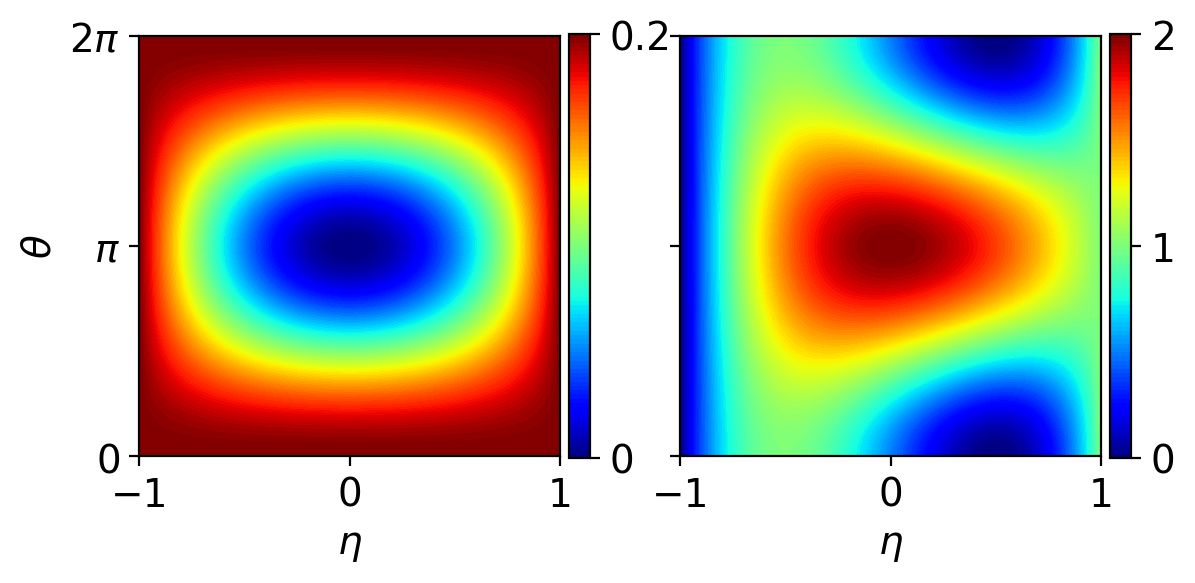
\includegraphics[width=0.8\textwidth]{gfx/ch-spin2/a20-a30-varying.png}
    \caption[Spin-singlet duo and trio amplitudes in a parameter space of
        \(\chi \) and \(\eta \)]
    {\label{fig: UN-BN-duo-trio} Spin singlet-duo (left) and -trio
        (right) amplitudes for the interpolating spinor in
        Eq.~\eqref{eq: UN-BN-interpolating-spinor}.
        Due to the spatially-dependent \(\eta \), this spinor continuously
        interpolates between the UN, BN, and cyclic phases depending on the
        relative phase difference \(\chi=\chi_2+\chi_{-2}-2\chi_0\).}
\end{figure}
Upon investigation, we see interesting behaviour arise in both quantities.
In particular, we see that this spinor can interpolate between the different
phases of UN, BN and cyclic depending on both \(\eta \) and the relative phase
difference \(\chi \).
For example, if one were to maintain \(\theta=0\) and interpolate \(\eta \),
then there would be multiple transitions between the UN (\(|A_{20}|^2 = 1\)) and
BN (\(|A_{20}|^2 = 0\)) phases.
In addition, maintaining a relative phase difference of \(\chi=\pi \), the
singlet-trio amplitude reveals that a cyclic phase is present when
\(-0.5 \lesssim \eta \lesssim 0.5\).
As we shall see in our numerical investigations, this has profound effects on
the structure of topological defects connecting across such an interface.

To begin our investigations of defects connecting across topological interfaces,
we first consider vortex connections.
A summary of different vortex connections possible across a UN-BN interface are
listed in Table~\ref{tab: UN-BN-vortices}.
\begin{table}
    \centering
    \begin{tabular}{cccccc}
        \toprule
        \multicolumn{5}{c}{Uniaxial nematic to biaxial nematic (UN-BN) ---
        Vortices} \\
        \midrule
        UN limit & BN limit &  \(\chi_2/\varphi \) & \(\chi_0/\varphi \) &
        \(\chi_{-2}/\varphi \)  \\
        \midrule
         Singular phase vortex & Singular phase vortex & \(k\) & \(k\) &
         \(k\) \\ 
         Vortex-free & Singular phase vortex & \(k\) & 0 & \(k\) \\
         Singular phase vortex & Vortex-free & 0 & \(k\) & 0\\
         Vortex-free & Singular spin vortex  & \(-k\) & 0 & \(k\) \\
         Singular phase vortex & Singular spin vortex  & \(-k\) & \(k\) &
         \(k\) \\
         Vortex-free & Half-quantum vortex  & \(k\) & 0 & 0\\
         Singular phase vortex & Half-quantum vortex  & \(k\) & \(k\) & 0 \\
        \bottomrule
    \end{tabular}
    \caption{\label{tab: UN-BN-vortices}
    Representative examples of different vortex connections possible across a
    UN-BN interface, constructed from the winding of the phase coefficients
    \(\chi_m\) in Eq.~\eqref{eq: UN-BN-interpolating-spinor}.
    Additionally, generalisations to multiply quantised vortices are given by
    \(k \in \mathbb{Z}\).}
\end{table}
We start by constructing a connection of singly quantised vortices (SQVs) on
either side of the interface, which can be achieved by allowing
\(\chi_m=\varphi \) in Eq.~\eqref{eq: UN-BN-interpolating-spinor}, which results
in a spatially overlapping \(2\pi \) phase winding in each component.
An alternative construction is achieved using
Eq~\eqref{eq: general-defect-interface}, where instead \(\tau=\varphi \) and the
Euler angles are kept constant.
Such a spinor is given explicitly as
\begin{align}\label{eq: UN-BN-SQV-SQV}
    \zeta_\text{sqv-sqv}^\text{UN-BN} =
    \frac{1}{2}\mqty(
        e^{i\varphi}\sqrt{1-\eta} \\
        0 \\
        e^{i\varphi}\sqrt{2(1+\eta)} \\
        0 \\
        e^{i\varphi}\sqrt{1-\eta}
    ).
\end{align}
One can see that in the above spinors we recover the individual SQV case in both
the UN \(\zeta^\text{UN}_\text{sqv} = {(0,0,e^{i\varphi},0,0)}^T\) and BN
\(\zeta^\mathrm{BN}_\text{sqv} ={(e^{i\varphi},0,0,0,e^{i\varphi})}^T/\sqrt{2}\)
limits when \(\eta = \pm 1\), respectively.
It is important to note that, despite being characterised by the same phase
winding, the SQVs on either side of the interface represent entirely different
objects due to the differing topologies of the UN and BN phases.

Instead of connecting two vortices on either side of the interface, one can
instead construct a vortex that terminates on the interface itself, essentially
connecting to a vortex-free region on the other side.
This can be achieved by selectively removing the phase winding from particular
components.
For example, to achieve an SQV in the UN limit that connects to a vortex-free
region in the BN limit, we can set \(\chi_0 = 0\) and \(\chi_{\pm 2}
= \varphi \) in Eq.~\eqref{eq: UN-BN-interpolating-spinor}, which gives
\begin{align}\label{eq: UN-BN-sqv-vf}
    \zeta^\text{UN-BN}_\text{sqv-vf} = \frac{1}{2}\mqty(
        \sqrt{1-\eta} \\
        0 \\
        e^{i\varphi} \sqrt{2(1+\eta)} \\
        0 \\
        \sqrt{1-\eta}
    ).
\end{align}
Similarly, by reversing this and setting the winding \(\chi_{\pm 2} = 0\) and
\(\chi_0=\varphi \) one instead constructs an SQV in the BN phase which connects
to a vortex-free region in the UN limit, given by the spinor
\begin{align}\label{eq: UN-BN-vf-sqv}
    \zeta^\text{UN-BN}_\text{vf-sqv} = \frac{1}{2}\mqty(
        e^{i\varphi} \sqrt{1-\eta} \\
        0 \\
        \sqrt{2(1+\eta)} \\
        0 \\
        e^{i\varphi} \sqrt{1-\eta}
    ).
\end{align}

One can use the above spinors to not just model the topological interface in the
bulk condensate, but also model the inside of the vortex
cores~\cite{Lovegrove2016, Weiss2019}.
For example, consider that \(\eta \) now has a radial dependence, with the
radial distance given as \(\rho = \sqrt{x^2 + y^2}\).
The particular case of Eq.~\eqref{eq: UN-BN-sqv-vf} can be modelled by requiring
\(\eta(0) = -1\), and \(\eta(\rho)\) interpolates to \(\eta(\rho) = 1\) away
from the vortex core, where we assume the vortex to be located at \(\rho = 0\).
This then results in the core taking on the BN phase, which smoothly
interpolates back to the UN phase far from the vortex core.
In addition, the phase difference arising between the components becomes
\(\chi = \mp 2\varphi \) for Eq~\eqref{eq: UN-BN-sqv-vf} and
Eq~\eqref{eq: UN-BN-vf-sqv}, respectively, which implies that \(\chi \) can take
values between 0 and \(4\pi \) about the vortex line.
Comparing this with Fig.~\ref{fig: UN-BN-duo-trio}, we see that at some point
this phase difference will cross \(\chi = \pi \) (and also \(\chi=3\pi \)) in a
region about the interface (\(\eta = 0\)), which implies that, interestingly, a
transition to the cyclic phase will occur within the vortex cores.
This results in an interface forming within the vortex core itself, containing
the BN, UN, and cyclic phases.
Such a vortex core interface is investigated in
Sec.~\ref{subsec: UN-BN-numerics}.

Vortices other than singular phase vortices may also be connected across the
interface.
One such example is of singular spin vortices, which, allowing for the fact that
spinor BECs support the non-dissipative flow of spin, carry a circulation only
in the condensate spin and not the mass (see Sec.~\ref{sec: vortices-spin-2}).
An example can be constructed by considering opposite phase windings in the
outer components, i.e., choosing \(\chi_{\pm 2} = \pm \varphi \) in
Eq.~\eqref{eq: UN-BN-interpolating-spinor}, resulting in the spinor
(see Sec.~\ref{sec: vortices-spin-2})
\begin{align}\label{eq: UN-BN-vf-sv}
    \zeta_\text{vf-sv}^\text{UN-BN} = \frac{1}{2}\mqty(
        e^{i\varphi}\sqrt{1 - \eta} \\
        0 \\
        \sqrt{2(1+\eta)} \\
        0 \\
        e^{-i\varphi}\sqrt{1 - \eta}
    ).
\end{align}
Notice that there is no phase winding apparent in the above equation, which
implies that the spin vortex exists only within the BN limit, and therefore
smoothly connects to a vortex-free state in the UN limit.
It is, however, possible to construct a spin vortex on both sides of the
interface.
This can be achieved by first applying a spin rotation to the state initial
interpolating spinor in Eq.~\eqref{eq: UN-BN-interpolating-spinor}, i.e.,
applying Eq.~\eqref{eq: spin-2-rotation-matrix} with \(\beta = \pi/2\) and
keeping the Euler angles \(\alpha, \gamma \) constant.
Then, by again choosing \(\chi_{\pm 2} = \pm \varphi \), we arrive at the
resulting interpolating spinor (\(\alpha = \gamma = 0\)):
\begin{align}\label{eq: UN-BN-sv-sv}
    \zeta_\text{sv-sv}^\text{UN-BN} = \frac{1}{4}\mqty(
        e^{i\varphi}(\sqrt{1 - \eta} + \sqrt{3(1+\eta)}) \\
        0 \\
        \sqrt{6(1-\eta)} - \sqrt{2(1+\eta)} \\
        0 \\
        e^{-i\varphi}(\sqrt{1 - \eta} + \sqrt{3(1+\eta)})
    ).
\end{align}
The result of the initial spin rotation means that in the UN (\(\eta = 1\)) and
BN (\(\eta = -1\)) limits we now have a three-component spinor given by
\(\zeta^\text{UN}_\text{sv} = {(e^{i\varphi}\sqrt{6}, 0, 2, 0,
e^{-\varphi}\sqrt{6})}^T/4\) and
\(\zeta^\text{BN}_\text{sv} = {(e^{i\varphi}\sqrt{2}, 0, 2\sqrt{3}, 0,
e^{-\varphi}\sqrt{2})}^T/4\), respectively, thereby allowing spin vortices to
appear in both phases, and hence connect across the topological interface.

So far, we have considered only singular vortices connecting across the
interface.
It is, however, possible to construct interpolating solutions that contain
higher order defects, such as monopoles and nonsingular textures.
To construct these, we generate the most general UN-BN interpolating spinor,
which is obtained by substituting Eq.~\eqref{eq: UN-BN-interpolating-spinor}
into Eq.~\eqref{eq: general-defect-interface} with arbitrary Euler
angles, which yields
\begin{align}\label{eq: UN-BN-general}
    \zeta^\text{UN-BN}=\frac{1}{\sqrt{2}}\left(
        \sqrt{1+\eta}\zeta^\text{UN}_\text{ns} + 
        \sqrt{1-\eta}\zeta^\text{BN}_\text{ns}
        \right),
\end{align}
where the UN and BN single phase limits are given, respectively, as
\begin{align}\label{eq: UN-general}
    \zeta^\text{UN}_\text{ns} &= \sqrt{\frac{3}{8}}
    \mqty(
        e^{-2i\alpha}\sin^2\beta \\
        e^{-i\alpha}\sin 2 \beta \\
        \frac{1}{\sqrt{6}}\left(1+3\cos 2\beta\right) \\
        -e^{i\alpha} \sin 2 \beta \\
        e^{2i\alpha}\sin^2\beta
    ), \\
    \zeta^\text{BN}_\text{ns} &= \frac{1}{\sqrt{8}} \label{eq: BN-general}
    \mqty(
        e^{-2i\alpha}\left(\cos^2\beta + 1\right) \\
        - e^{-i\alpha}\sin 2 \beta \\
        \sqrt{6}\sin^2\beta \\
        e^{i\alpha}\sin 2 \beta \\
        e^{2i\alpha}\left(\cos^2\beta + 1\right)          
    ).
\end{align}
An interesting example can be constructed by thinking about a monopole placed in
the UN limit, which can be realised from a spherically symmetric dependence
on the nematic director, \(\hat{\vb{d}} = (\cos\alpha \sin\beta, \sin\alpha
\sin\beta, \cos\beta)\).
A monopole can be constructed in the UN phase from Eq.~\eqref{eq: UN-general}
by choosing \(\alpha=\varphi \) and having \(\beta = \theta \), where
\(\theta \) is the polar angle in spherical coordinates.
Using the same choice for the BN limit in Eq.~\eqref{eq: BN-general} also
results in a monopole, despite such a monopole not being stable in the BN phase
(i.e., the second homotopy group of the BN order parameter space is zero).

A type of nonsingular vortex arising in both the UN and BN limits is that of the
nematic coreless vortex which carry zero angular
momentum~\cite{Choi2012, Lovegrove2014}.
A connection between nematic coreless vortices is achieved by setting
\(\alpha=\varphi \) and by having a radially-dependent Euler angle
\(\beta(\rho)\) in Eq.~\eqref{eq: UN-BN-general}, where \(\beta(0)=0\)
on the vortex line, monotonically increasing to \(\beta(\rho=\pi/2)\) far from
the vortex.
A summary of other types of defects one can obtain in a UN-BN interface is
given in Table~\ref{tab: UN-BN-nonsingular}.
\begin{table}
    \centering
    \begin{tabular}{cccccc}
        \toprule
        \multicolumn{6}{c}{Uniaxial nematic to biaxial nematic ---
        Other defects/textures} \\
        \midrule
        UN limit & BN limit &  \(\tau/\varphi \) & \(\alpha/\varphi \) &
        \(\gamma/\varphi \) & \(\beta \) \\
        \midrule
        Monopole & Monopole & 0 & \(k\)  & 0 & \(k\theta \) \\
        Nonsingular vortex & Nonsingular vortex & 0 & 1 & 0 &
        \(\beta(\rho)\) \\ 
        \bottomrule
    \end{tabular}
    \caption{\label{tab: UN-BN-nonsingular}
    Summary of other types of defect connections possible in a UN-BN interface.
    Given solutions are characterised by winding of the condensate phase,
    \(\tau \), and Euler angles (\(\alpha, \beta, \gamma \)), expressed in units
    of the azimuthal angle \(\varphi \).
    Here, \(k\) is an integer which provides a generalisation to higher
    quantisation.
    Additionally, \(\theta \) is the polar angle in spherical coordinates, and
    \(\beta(\rho)\) describes a monotonically increasing function of the
    transverse radius \(\rho \).}
\end{table}

\subsection{Cyclic to nematic}
As we have discussed already in the context of vortex cores, topological
interfaces can arise between the cyclic and nematic phases.
From Fig.~\ref{fig: UN-BN-duo-trio}, we see that by maintaining a constant
\(\chi=\pi \) one can interpolate between the UN, cyclic and BN states.
This can be achieved by the following family of spinors
\begin{align}\label{eq: C-N-interpolating-spinor}
    \zeta^\text{C-N} = \frac{1}{2}\mqty(
    e^{i\chi_2}\sqrt{1 - \eta} \\
    0 \\
    ie^{i\chi_0}\sqrt{2(1+\eta)} \\
    0 \\
    e^{i\chi_{-2}}\sqrt{1 - \eta}
    ),
\end{align}
where we now require that \(\chi_2 + \chi_{-2} - 2\chi_0 = 0\).
Then, due to the \(i\) term in the middle component, this leads to a constant
phase difference of \(\chi_2 + \chi_{-2} - 2(\chi_0 + \pi/2) = -\pi \), and
hence allows us to use the quadratic Zeeman shift to interpolate the above
solution between the different phases.
At \(\eta = 0\) the above solution becomes the three component cyclic state with
a spinor of the form \(\zeta_\mathrm{C} = {(1, 0, i\sqrt{2}, 0, 1)}^T/2\).
The sign of the quadratic Zeeman shift determines which nematic state is chosen,
where \(\eta = \pm 1\) recovers the familiar UN and BN states, respectively.

The uniform mean-field energy of Eq.~\eqref{eq: C-N-interpolating-spinor} reads
\begin{equation}
    E^\text{C-N} = \frac{c_2n}{10}\eta^2 + 2q(1 - \eta).
\end{equation}
The energy becomes minimised at \(\eta = 10q/c_2n\) for \(c_2 > 0\) and fixed
\(q\).
Since the interpolating spinor \(\zeta^\text{C-N}\) is a function of \(q\) only,
the stability of the interface is guaranteed since \(E^\text{C-N} =
2q-10q^2/c_2 \leq E^\text{C}, E^\text{UN},
E^\text{BN}\) for \(|q| < c_2n/10\).
Here, for simplicity, we focus on an interface between the cyclic and BN phases
which is achieved from a longitudinally-dependent quadratic Zeeman shift
\(q(z)\) which varies from \(q = 0\) at the cyclic phase to \(q = -c_2n/10\)
at the BN side.

Firstly, one can construct the same SQV and spin vortex connections considered
in the UN-BN interface upon the substitution \(\sqrt{1+\eta} \rightarrow
i\sqrt{1+\eta}\) in Eqs.~\eqref{eq: UN-BN-SQV-SQV} and~\eqref{eq: UN-BN-sv-sv},
identifying the cyclic limit as \(\eta = 0\).
However, choosing the phase windings \(\chi_m\) such that \(\chi \neq 0\) leads
to defect states which are undefined in the cyclic limit, and hence we omit
them from the discussion.
These defect states are summarised in Table~\ref{tab: C-N-vortices}.
\begin{table}
    \centering
    \begin{tabular}{cccccc}
        \toprule
        \multicolumn{6}{c}{Cyclic to nematic --- vortices} \\
        \midrule
        Cyclic limit & UN limit & BN limit & \(\chi_2/\varphi \) &
        \(\chi_0/\varphi \) & \(\chi_{-2}/\varphi \) \\
        \midrule
            SQV & SQV & SQV & \(k\) & \(k\) & \(k\) \\
            Singular spin vortex & Vortex-free & Singular spin vortex & \(-k\)
            & 0 & \(k\) \\
        \bottomrule
    \end{tabular}
    \caption{\label{tab: C-N-vortices}Summary of the phase and spin vortices
    possible in a cyclic to nematic interface.
    Different vortices are constructed from appropriate choices of the phase
    windings \(\chi_m\).
    Note that \(\chi=0\) for all cases considered as to
    ensure identifiable vortices within the cyclic limit.}
\end{table}

In addition to these connections, it is also possible to construct topologically
distinct spin vortex connection between the cyclic and both nematic phases.
This arises from the common axis of symmetry between the cyclic and BN phases
(see \(C_2'\) axis in Fig.~\ref{fig: spin-2-spherical-harmonics}d).
A spin rotation around this particular axis can be achieved from the spin-2
rotation matrix in Eq.~\eqref{eq: spin-2-rotation-matrix} by choosing
\(\alpha = -\gamma =\pi / 4\) and keeping \(\beta \) arbitrary.
Applying the transformation in Eq.~\eqref{eq: general-defect-interface} to the
general cyclic to nematic spinor in Eq.~\eqref{eq: C-N-interpolating-spinor}
using these Euler angles with \(\tau=0\) and \(\beta = \varphi \) results in
the following spinor:
\begin{align}
    \zeta^\text{C-N}_\mathrm{sv-sv} = \frac{1}{\sqrt{2}}\left(
    i\sqrt{1+\eta}\zeta^\mathrm{UN}_\mathrm{sv} +
    \sqrt{1-\eta}\zeta^\mathrm{BN}_\mathrm{sv}
    \right), \label{eq: C-BN-sv-sv}
\end{align}
where the spin vortices in the UN and BN limits are given as
\begin{gather}
    \zeta^\mathrm{UN}_\mathrm{sv} = \sqrt{\frac{3}{8}}
    \mqty(
    \sin^2 \varphi \\
    e^{\frac{i\pi }{4}} \sin 2\varphi \\
    \frac{i}{\sqrt{6}}\left(1 + 3\cos 2\varphi \right)\\
    e^{-\frac{i \pi }{4}} \sin2 \varphi \\
    -\sin^2 \varphi
    ), \\
    \zeta^\mathrm{BN}_\mathrm{sv} = \frac{1}{\sqrt{2}}
    \mqty(
    \cos \varphi \\
    e^{-\frac{3i\pi }{4}} \sin \varphi \\
    0\\
    e^{-\frac{i \pi }{4}} \sin \varphi \\
    \cos \varphi
    ).
\end{gather}
This yields a connection between an integer spin vortex in the cyclic limit to
another integer spin vortex in both nematic limits.

As discussed in the previous section, the nematic phases give rise to
nonsingular textures and point defects such as nematic coreless vortices and
monopoles.
Those same defect connections can be constructed in this interface by using
the appropriate transformation \(\sqrt{1+\eta} \rightarrow i\sqrt{1+\eta}\) in
Eq.~\eqref{eq: UN-BN-general}.
This then still results in, for example, the nematic coreless vortices in the
nematic limits, which now connect to a nonsingular vortex structure in the
cyclic limit.
These defects are summarised in Table~\ref{tab: C-N-other}.
\begin{table}
    \centering
    \begin{tabular}{cccccc}
        \toprule
        \multicolumn{6}{c}{Cyclic to nematic --- Other defects/textures} \\
        \midrule
        Cyclic limit & UN/BN Limits &  \(\tau/\varphi \) & \(\alpha/\varphi \)
        & \(\gamma/\varphi \) & \(\beta \) \\
        \midrule
         Singular spin vortex & Singular spin vortex & 0 &
         \(\alpha=\frac{\pi}{4}\) & \(\gamma=-\alpha \) & \(k\varphi \) \\
         Nonsingular vortex & Nonsingular vortex & 0 & 1 & 0
         & \(\beta(\rho)\) \\ 
         Monopole & Monopole & 0 & \(k\)  & 0 & \(k\theta \) \\
        \bottomrule
    \end{tabular}
    \caption{\label{tab: C-N-other}Summary of other types of defect structures
    possible in a cyclic to nematic interface.
    Each defect is identified by windings of the condensate phase \(\tau \) and
    Euler angles (\(\alpha, \beta, \gamma \)), expressed in terms of the
    azimuthal angle \(\varphi \).
    For nonsingular vortices, \(\beta(\rho)\) denotes a monotonically increasing
    function of the transverse radius \(\rho \).
    Additionally, for the monopole case, \(\theta \) is the polar angle in
    spherical coordinates.}
\end{table}

\subsection{Cyclic to ferromagnetic}
Since spin-2 BECs support a ferromagnetic phase, which has inherent
magnetisation, it is natural to construct an interface between this state and
one with zero magnetisation.
This would then result in spatially distinct regions which have different values
of the spin magnitude, and hence would create a spatially-dependent
magnetisation.
By restricting ourselves to the case of zero transverse magnetisation,
\(\hat{\vb{F}} = \hat{F}_z\), one such case that arises is between the cyclic
and ferromagnetic phases, given by the following family of spinors:
\begin{align}\label{eq: C-FM-interpolating-spinor}
    \zeta^\text{C-FM} = \frac{1}{\sqrt{3}}\mqty(
        e^{i\chi_2}\sqrt{1 + \eta} \\
        0 \\
        0 \\
        e^{i\chi_{-1}}\sqrt{2 - \eta} \\
        0
    ),
\end{align}
where \(\eta \) now becomes the longitudinal magnetisation, \(\hat{F}_z\).
At zero magnetisation, \(\hat{F}_z = 0\), equivalent to setting \(\eta=0\), this
solution becomes the two-component cyclic state,
\(\zeta^C = {(1, 0, 0, \sqrt{2}, 0)}^T/\sqrt{3}\) which naturally has no
magnetisation.
Then, since this is a spin-2 system, the condensate spin is free to vary between
\(\hat{F}_z = 0\) and \(\hat{F}_z = 2\).
Recall from Chapter~\ref{chap: ground-states} that the spin-2 system supports
two FM ground states, one with \(\spinmag = 1\), which we denote
FM-1, and another with \(\spinmag = 2\), which we denote FM-2.
Therefore, this spinor can interpolate between the cyclic and both FM phases,
depending on the value of the condensate spin, \(\hat{F}_z\).

The uniform mean-field energy of the above spinor reads
\begin{equation}
    E^\text{C-FM} = \frac{c_1 n}{2} \eta^2 - (p-q)\eta + 2q,
\end{equation}
which becomes minimised upon the choice \(\eta = (p-q)/c_1n\) for \(c_1 > 0\)
and fixed \(p, q\).
The interface is expected to be stable within the range
\(-c_1n \leq p \leq 2c_1n\) since \(E^\text{C-FM} \leq
E^\text{C}=0, E^{f_z=1} = c_1n/2 + p\).
Therefore, assuming, e.g., \(q=0\), we can stabilise the interface by an
appropriate choice of a longitudinally-dependent linear Zeeman shift \(p(z)\),
where \(p(z) = 0\) represents the cyclic phase, whilst \(p(z) = -c_1n\) and
\(p(z) = 2c_1n\) represent the FM-1 and FM-2 phases,
respectively.

Following the procedure similar to the previous interfaces, we first focus on
constructing phase vortices connecting across this topological interface, which
can be obtained by appropriate winding of \(\chi_2\) and \(\chi_{-1}\).
Again, one can construct singular SQVs connecting in all three limits by
crossing \(\chi_2 = \chi_{-1} = \varphi \), which yields
\begin{align}\label{eq: C-FM-sqv-sqv}
    \zeta^\text{C-FM}_\text{sqv-sqv} = \frac{e^{i\varphi}}{\sqrt{3}}\mqty(
        \sqrt{1 + \eta} \\
        0 \\
        0 \\
        \sqrt{2 - \eta} \\
        0
    ),
\end{align}
In addition to these singly quantised vortices, the cyclic phase supports
vortices with fractional charges, such as one-third and two-third vortices (see
Sec.~\ref{sec: vortices-spin-2}).
One can then construct such a vortex in the cyclic limit by limiting the winding
of the phase to only one component.
Due to the spin-gauge symmetry of the FM phase, this choice of winding would
then lead to either singular SQVs and vortex-free regions in this limit.
For example, the following spinor connects a one-third vortex in the cyclic
limit to a singular SQV in the FM-2 and a vortex-free region in the FM-1 limit:
\begin{align}\label{eq: C-FM-third-sqv}
    \zeta^\text{C-FM}_\text{third-sqv} = \frac{1}{\sqrt{3}}\mqty(
        e^{i\varphi}\sqrt{1 + \eta} \\
        0 \\
        0 \\
        \sqrt{2 - \eta} \\
        0
    ),
\end{align}
which corresponds to the choice of \(\chi_2 = \varphi \) and \(\chi_{-1} = 0\)
in Eq.~\eqref{eq: C-FM-interpolating-spinor}.
Similarly, a two-third vortex in the cyclic limit can connect to a vortex-free
region in the FM-2 limit or a singular SQV in the FM-1 limit, given by the
spinor
\begin{align}\label{eq: C-FM-2third-vf}
    \zeta^\text{C-FM}_\text{two-third-sqv} = \frac{1}{\sqrt{3}}\mqty(
        e^{i\varphi}\sqrt{1 + \eta} \\
        0 \\
        0 \\
        \sqrt{2 - \eta} \\
        0
    ),
\end{align}
equivalent to setting \(\chi_2 = 0\) and \(\chi_{-1}=\varphi \) in
Eq.~\eqref{eq: C-FM-interpolating-spinor}.
Note that equivalent constructions can be made for the above two spinors using
Eq.~\eqref{eq: general-defect-interface} with \(\tau=-\gamma=\varphi/3\) and
\(\tau=2\gamma=2\varphi/3\), respectively.
A summary of the phase vortex connections possible in this interface are
summarised in Table~\ref{tab: C-FM-vortices}.
\begin{table}
    \centering
    \begin{tabular}{ccccc}
        \toprule
        \multicolumn{5}{c}{Cyclic to ferromagnetic --- Vortices} \\
        \midrule
        C limit & FM-2 limit & FM-1 limit & \(\chi_2/\varphi \)
        & \(\chi_{-1}/\varphi \) \\
        \midrule
         SQV & SQV & SQV & \(k\) & \(k\) \\ 
         One-third & SQV & Vortex-free & \(k\) & 0 \\
         Two-third vortex & Vortex-free & SQV & 0 & \(k\) \\
         Singular spin vortex & Singular spin vortex & Singular spin vortex
         & \(-2k\) & \(k\) \\
        \bottomrule
    \end{tabular}
    \caption{\label{tab: C-FM-vortices}Summary of the vortex connections
    possible in a cyclic to FM interface.
    Each vortex can be constructed by choosing the appropriate phase winding
    \(\chi_m\), expressed in terms of the azimuthal angle \(\varphi \).
    Here, \(k \) is an integer that allows one to represent vortices of
    arbitrary quantisation.
    Note that, for example, choosing \(k=3\) would result in a one-third
    vortex now having unit quantisation, but it would be topologically distinct
    to the SQV constructed from the choice \(\chi_2=\chi_{-1}=k\).}
\end{table}

In addition to phase vortices, the FM phase also supports nonsingular coreless
vortices, which is identified from a characteristic fountain-like texture of
the condensate spin (see Fig.~\ref{fig: spin-1-vortices}b for the spin-1
analogue.)
To construct such a defect across an interface, we make use of
Eq.~\eqref{eq: general-defect-interface}, and apply it to the general cyclic to
FM interface in Eq.~\eqref{eq: C-FM-interpolating-spinor}.
To construct the characteristic fountain-like spin texture, we choose a
monotonically increasing function of \(\beta=\beta(\rho)\).
The order-parameter is then kept single-valued by a combined winding of the
condensate phase coupled to a winding of the spin vector, achieved by
\(\tau'=2\alpha=2\varphi \), where \(\tau'=\tau-2\gamma \).
This then results in the spinor
\begin{equation}\label{eq: C-FM-coreless-general}
    \zeta_\text{cl} = \frac{1}{\sqrt{3}}\left(
        \sqrt{1 + \eta}\zeta^\text{FM-2}_\text{cl}
        + \sqrt{2 - \eta}\zeta^\text{FM-1}_\text{cl}\right),
\end{equation}
where
\begin{align}\label{eq: C-FM-coreless-FM-limits}
    \zeta^\text{FM-2}_\text{cl} =
    \mqty(
    \cos^4\frac{\beta(\rho)}{2}                                        \\
    2e^{i\varphi}\cos^3\frac{\beta(\rho)}{2}\sin\frac{\beta(\rho)}{2}  \\
    \sqrt{6}e^{2i\varphi}\cos^2\frac{\beta(\rho)}{2}\sin^2
    \frac{\beta(\rho)}{2}                                              \\
    2e^{3i\varphi}\cos\frac{\beta(\rho)}{2}\sin^3\frac{\beta(\rho)}{2} \\
    e^{4i\varphi}\sin^4\frac{\beta(\rho)}{2}
    ),
\end{align}
\begin{align}
    \zeta^\text{FM-1}_\text{cl} =
    \mqty(
    -2\cos\frac{\beta(\rho)}{2}\sin^3\frac{\beta(\rho)}{2}         \\
    e^{i\varphi}\sin^2\frac{\beta(\rho)}{2}\left(3\cos^2
    \frac{\beta(\rho)}{2}-\sin^2\frac{\beta(\rho)}{2}\right)       \\
    \sqrt{6}e^{2i\varphi}\left(\cos\frac{\beta(\rho)}{2}\sin^3
    \frac{\beta(\rho)}{2}
    - \cos^3\frac{\beta(\rho)}{2}\sin\frac{\beta(\rho)}{2} \right) \\
    e^{3i\varphi}\cos^2\frac{\beta(\rho)}{2}\left(\cos^2
    \frac{\beta(\rho)}{2}-3\sin^2\frac{\beta(\rho)}{2}\right)      \\
    2e^{4i\varphi}\cos^3\frac{\beta(\rho)}{2}\sin\frac{\beta(\rho)}{2}
    )
\end{align}
represent coreless vortices in both the FM-2 and FM-1 limits, respectively.
The spherical harmonic representation of these coreless vortices are shown
in Fig.~\ref{fig: C-FM-coreless-initial-states}a,
~\ref{fig: C-FM-coreless-initial-states}b, where we see the characteristic
fountain-like texture emerge.
\begin{figure}
    \centering
    \begin{tikzpicture}
        \node at (0, 0) {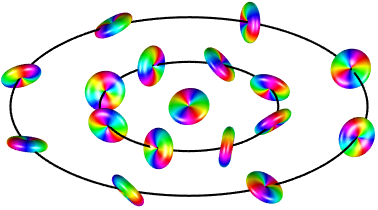
\includegraphics[width=0.45\textwidth]
            {gfx/ch-spin2/C-FM=2_coreless_FM_init_spherical.pdf}};
        \node at (7.5, 0) {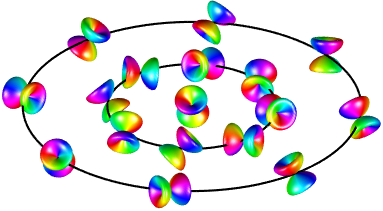
\includegraphics[width=0.45\textwidth]
            {gfx/ch-spin2/FM-1_coreless_init_state.pdf}};
        \node at (3.75, -4) {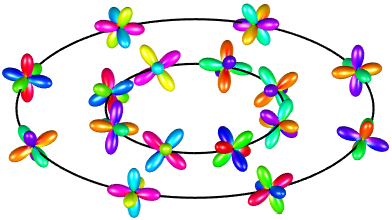
\includegraphics[width=0.45\textwidth]
            {gfx/ch-spin2/C-FM=2_coreless_cyclic_init_spherical.pdf}};

        % Colour bar
        \node at (3.25, 2.3){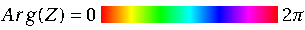
\includegraphics{gfx/colourbars/compiled_hsv.pdf}};

        % Labels
        \node at (0, -2.2) {(a)};
        \node at (7.5, -2.2) {(b)};
        \node at (3.75, -6.2) {(c)};
    \end{tikzpicture}
    \caption[Spherical harmonic representation of a coreless vortex connection
        across a cyclic to ferromagnetic interface]
    {\label{fig: C-FM-coreless-initial-states}Spherical harmonic
        representation of the topological defects obtained in the cyclic, FM-1,
        and FM-2 limits in Eq.~\eqref{eq: C-FM-coreless-general}.
        (a) and (b): Coreless vortex in the FM-2 and FM-1 limit, respectively,
        given by Eq.~\eqref{eq: C-FM-coreless-FM-limits}.
        (c): Doubly quantised vortex in the cyclic limit, given by
        Eq.~\eqref{eq: C-FM-DQV-cyclic-limit}.}
\end{figure}
The resulting spinor in the cyclic limit is
\begin{equation}\label{eq: C-FM-DQV-cyclic-limit}
    \zeta_\text{dqv}
    = \left(\zeta^\text{FM-2}_\text{cl}
    + \sqrt{2}\zeta^\text{FM-1}_\text{cl}\right) / 3,
\end{equation}
where the spherical harmonic representation of this cyclic state is plotted in
Fig.~\ref{fig: C-FM-coreless-initial-states}c.
By tracing a point about the vortex core, the condensate phase winds by a total
of \(4\pi \), coupled with a non-trivial rotation of the condensate spin,
indicating that this is particular vortex is a doubly-quantised vortex.
Therefore, the interpolating spinor above connects FM coreless vortices to a
doubly-quantised vortex in the cyclic limit.

\subsection{Ferromagnetic to biaxial nematic}
Another interface containing non-zero magnetisation is that between the FM and
BN phases, given by the following family of spinors:
\begin{align}\label{eq: FM-BN-interpolating-spinor}
    \zeta^\text{FM-BN} = \frac{1}{\sqrt{2}}\mqty(
    e^{i\chi_2} \sqrt{1 + \eta} \\
    0 \\
    0 \\
    0 \\
    e^{i\chi_{-2}} \sqrt{1 - \eta}),
\end{align}
where \(\eta \) relates to the longitudinal magnetisation as \(\eta =
\hat{F}_z / 2\).
This state then interpolates between the BN state at \(\eta = 0\), to an FM
state with spin pointing up (down) for \(\eta = 1 (-1)\).
The energy of this interpolating spinor is obtained by substituting the above
into Eq.~\eqref{eq: energy-per-particle}, which reads
\begin{align}\label{eq: FM-BN-energy}
    E^\text{FM-BN} = \frac{n}{2}\left(c_1-\frac{c_2}{20}\right)\eta^2
    - p \eta + 4q + \frac{nc_2}{10}.
\end{align}
This energy becomes minimised precisely when \(\eta = p / [(c_1-c_2/20)n]\) for
\(c_1 \geq c_2/20\) and fixed \(p\) and \(q\).
Substitution of \(\eta = p / [(c_1-c_2/20)n]\) into Eq.~\eqref{eq: FM-BN-energy}
reveals that \(E^\text{FM-BN} \leq E^\text{BN},
E^{FM-2}\) for \(|p| < (2c_1-c_2/10)n\).
Thus, as in the previous FM interface, we can stabilise the interface by relying
on a longitudinal dependence of the linear Zeeman shift, \(p(z)\).
One can see that at \(p = \pm 2(c_1-c_2/20)n\) the above solution becomes
the ferromagnetic state with spin \(\eta = \pm 2\).
Alternatively, the solution becomes the BN state precisely when \(p=0\), and
hence has zero magnetisation.
Therefore, this spinor provides an interpolating solution between the
ferromagnetic and BN phases, which is controlled by a longitudinal dependence of
the linear Zeeman shift, \(p(z)\).

We start from the interpolating spinor between the FM and BN phases in
Eq.~\eqref{eq: FM-BN-interpolating-spinor} and first construct various vortex
states using different combinations of the phase windings \(\chi_{\pm 2}\).
Again, similar to the previous cases, SQVs are connected across the interface
by the choice \(\chi_{\pm 2} = \varphi \).
An interesting case arises between a singular phase vortex in the FM phases
connecting to a spin vortex in the BN phase.
This can be achieved by again allowing opposite phase windings in the outer
components, i.e., \(\chi_{\pm 2} = \pm \varphi \), where the interpolating
spinor reads
\begin{align}\label{eq: FM-BN-sqv-sv}
    \zeta^\text{FM-BN}_\text{sqv-sv} = \frac{1}{\sqrt{2}}\mqty(
    e^{i\varphi} \sqrt{1 + \eta} \\
    0 \\
    0 \\
    0 \\
    e^{-i\varphi} \sqrt{1 - \eta}).
\end{align}

As observed in Fig.~\ref{fig: SV-HQV}, the BN phase allows for the creation
of a HQV, characterised by a half-winding of the condensate phase.
Such a vortex can be constructed by allowing a phase winding in only one of the
outer components, i.e., \(\chi_2 = \varphi \) and \(\chi_{-2} = 0\) or vice
versa.
Using this first choice in Eq.~\eqref{eq: FM-BN-interpolating-spinor} leads to
the spinor
\begin{align}\label{eq: FM-BN-sqv-hqv}
    \zeta^\text{FM-BN}_\text{sqv-sv} = \frac{1}{\sqrt{2}}\mqty(
    e^{i\varphi} \sqrt{1 + \eta} \\
    0 \\
    0 \\
    0 \\
    \sqrt{1 - \eta}),
\end{align}
which connects this HQV to an SQV in the FM-2 limit when \(\eta = 1\), or a
vortex-free state when \(\eta = -1\).
Choosing \(\chi_{\pm 2}\) the opposite way around would reverse this connection.
A summary of these vortex connections is provided in
Table~\ref{tab: FM-BN-vortices}.
\begin{table}
    \centering
    \begin{tabular}{ccccc}
        \toprule
        \multicolumn{5}{c}{Ferromagnetic to biaxial nematic --- Vortices} \\
        \midrule
        FM-2 (up) limit & FM-2 (down) limit & BN limit &  \(\chi_2/\varphi \)
        & \(\chi_{-2}/\varphi \)  \\
        \midrule
         SQV & SQV & SQV & \(k\) & \(k\) \\ 
         SQV & Vortex-free & Half-quantum vortex & \(k\) & 0 \\
         Vortex-free & SQV & Half-quantum vortex & 0 & \(k\) \\
         SQV & SQV & Singular spin vortex  & \(-k\) & \(k\) \\
        \bottomrule
    \end{tabular}
    \caption{\label{tab: FM-BN-vortices}
    Summary of possible vortex connections across an FM to BN interface.
    Each vortex is given in terms of the winding \(\chi_m\), given in multiples
    of the azimuthal angle \(\varphi \).
    The FM limits are specified by the direction of the condensate spin, where
    a spin pointing up denotes a spinor of the form
    \(\zeta={(1, 0, 0, 0, 0)}^T\), and a spin pointing down denotes a spinor of
    the form \(\zeta={(0, 0, 0, 0, 1)}^T\).
    Additionally, \(k\) is an integer that allows one to generalise to higher
    quantisation.}
\end{table}

We can also construct nonsingular defect crossing solutions using this interface.
Again, since the FM phase supports a nonsingular coreless vortex, we can follow
the same methodology as in the cyclic to FM interface and construct a coreless
vortex connecting across the interface.
We apply Eq.~\eqref{eq: general-defect-interface} to the general FM-BN spinor
in Eq.~\eqref{eq: FM-BN-interpolating-spinor}, and choose a monotonically
increasing function for the Euler angle \(\beta(\rho)\) with a transverse
radial dependence, together with \(\tau - 2\gamma = 2\alpha = 2\varphi \).
This leads to the interpolating spinor
(\(\gamma=0\))
\begin{align}\label{eq: FM-BN-coreless-dqv}
    \zeta^\text{FM-BN}_\text{cl-dqv} = \mqty(
    C^4\sqrt{1+\eta} + S^4\sqrt{1-\eta} \\
    2e^{i\varphi}\left[C^3S\sqrt{1+\eta}
        - CS^3\sqrt{1-\eta}\right] \\
    e^{2i\varphi}\sqrt{6}C^2S^2\left[\sqrt{1+\eta}
        + \sqrt{1-\eta} \right] \\
    2e^{3i\varphi}\left[CS^3\sqrt{1+\eta}
        - C^3S\sqrt{1-\eta}\right] \\
    e^{4i\varphi}\left[S^4\sqrt{1+\eta} + C^4\sqrt{1-\eta} \right]
    ),
\end{align}
where \(C \equiv \cos(\beta(\rho)/2)\) and \(S \equiv \sin(\beta(\rho)/2)\).
In the FM limit, one recovers the spin-2 coreless vortex given as (\(\eta=1\))
\begin{align}\label{eq: FM-BN-coreless}
    \zeta^\text{FM}_\text{cl} = \sqrt{2}\mqty(C^4 \\ 2e^{i\varphi}C^3S \\
    e^{2i\varphi}\sqrt{6}C^2S^2 \\ 2e^{3i\varphi}CS^3 \\ e^{4i\varphi}S^4
    ).
\end{align}
The spherical harmonic representation of this vortex is plotted in
Fig.~\ref{fig: C-FM-coreless-initial-states}, where the characteristic
fountain-like texture becomes apparent.
The spinor in the BN limit (\(f_z=0\)) reads
\begin{align}\label{eq: FM-BN-DQV}
    \zeta^\text{BN}_\text{dqv} = \mqty(
    C^4 + S^4 \\
    2e^{i\varphi}CS\left[C^2-S^2\right] \\
    2e^{2i\varphi}\sqrt{6}C^2S^2 \\
    2e^{3i\varphi}CS\left[S^2 - C^2\right] \\
    e^{4i\varphi}\left[C^4 + S^4\right]).
\end{align}
It is not immediately obvious from the form of the spinor the type of vortex
present on the BN side of the interface.
The spherical harmonics plotted in Fig.~\ref{fig: BN-DQV} reveal that, similar
to the cyclic case, this is also doubly quantised vortex in the BN limit, which
can be seen by tracing a point about the vortex line, showing the condensate
phase changes by a total of \(4\pi \).
\begin{figure}
    \centering
    \begin{tikzpicture}
        \node at (0, 0) {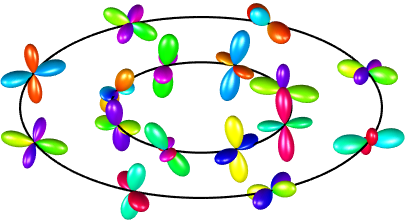
\includegraphics[width=0.5\textwidth]
            {gfx/ch-spin2/BN_DQV.pdf}};
        \node[cylinder, draw, fill=black, opacity=0.5, minimum height=4cm,
            rotate=90] (c_dqv) at (0, 0) {};

        % Colour bar
        \node[rotate=90] at (-4.15, 0.4)
        {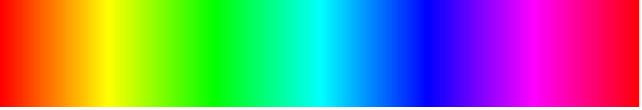
\includegraphics[width=0.15\textwidth, height=0.015\textheight]
            {gfx/colourbars/hsv_colourbar.pdf}};
        \node[rotate=90] at (-4.15, -1.6) {Arg(\(Z\)) = 0};
        \node[rotate=90] at (-4.15, 1.9) {\(2\pi \)};
    \end{tikzpicture}
    \caption[Spherical harmonic representation of a biaxial nematic doubly
        quantised vortex]
    {\label{fig: BN-DQV} Spherical harmonic
        representation of the BN vortex configuration given by
        Eq.~\eqref{eq: FM-BN-DQV}.
        A \(4\pi \) winding of the condensate phase about the core indicates
        this is a doubly quantised vortex, coupled with a non-trivial rotation
        of the condensate spin.}
\end{figure}

\section{Numerical investigations of defect crossing physics}
In this section we numerically investigate some topological interfaces defined
in the preceding section, along with a subset of the possible defect
connections.
Our numerical setup is as follows.
We numerically evolve the spin-2 GPEs defined in
Eqs.~\eqref{eq: spin-2-GPEs-pm2} -~\eqref{eq: spin-2-GPEs-0} using a symplectic
integrator~\cite{Symes2017} using, for simplicity, a purely isotropic trapping
potential \(V=M\omega^2r^2/2\).
We simulate the energy loss during experiments by introducing a phenomenological
damping coefficient, \(\nu \), through the substitution
\(t \rightarrow (1-i\nu)t\).
In all simulations considered, we choose \(\nu = 1e-2\).
We perform our simulations on a 3D of \(N_s^3=128^3\) points, with side lengths
\(L = 20\ell \), where \({(\ell =\hbar/M\omega)}^{1/2}\) is the (isotropic)
harmonic oscillator length.
We choose parameters that correspond to a \(^{87}\)Rb
condensate~\cite{Klausen2001} with \(c_0n=1.32\times10^4\hbar\omega\ell^3\),
\(c_0/c_1=90.7\), and \(c_0/c_2=-102\), where the ground state is predicted to
be nematic (see Sec.~\ref{subsec: spin-2-experimental-parameters} for details
on the choice of numerical parameters).
In each simulation, we perform a small spin rotation to the initial state to
avoid components that are identically zero.
Additionally, when constructing states with defects, the position of each defect
is perturbed slightly to avoid artificial stability when placed at exactly the
centre of the trap.
Details of the trapped, dimensionless units can be found in
Sec.~\ref{subsec: spin-2-dimensionless}.

\subsection{\label{subsec: UN-BN-numerics}
Uniaxial nematic to biaxial nematic interface}
The first interface we consider is that between the UN and BN phases, considered
in Sec.~\ref{subsec: UN-BN-defects}.
Since the UN and BN phases are energetically degenerate in the absence of a
magnetic field, we introduce a spatially-dependent quadratic Zeeman shift
\(q(z)\) such that \(q(z) > 0\) on the UN side and \(q(z) < 0\) on the BN side
to lift the degeneracy, and the maximum strength of our quadratic Zeeman shift
is set to \(q_\text{max} = 0.1\hbar\omega \).
The quadratic Zeeman shift linearly interpolates over a small transition region
(which we take to be small compared to the spin-dependent healing lengths) from
\(q = -0.1\hbar\omega \) in the BN phase to \(q = 0.1\hbar\omega \) in the UN
phase.

Our investigation begins with that of the SQV-SQV connection, where the initial
state is constructed as in Eq.~\eqref{eq: UN-BN-SQV-SQV}.
To imprint the vortices, we perform a short imaginary time propagation, then
proceed to numerically evolve the spin-2 GPEs.
The dynamics of this connection is split into two distinct parts, which are
plotted in Fig.~\ref{fig: UN-BN-SQV-SQV-singlets}.
Firstly, upon evolution, the two overlapping SQVs spatially separate due to an
instability occurring at the interface \(z \approx 0\).
Each SQV then connects to a vortex-free state on the other side of the
interface shown in Fig.~\ref{fig: UN-BN-SQV-SQV-singlets}a.
After the initial separation, the cores of the vortices fill with atoms
occupying different ground states, drastically altering the order parameter
symmetry within the cores.
\begin{figure}
    \centering
    \begin{tikzpicture}
        \node at (0, 0) {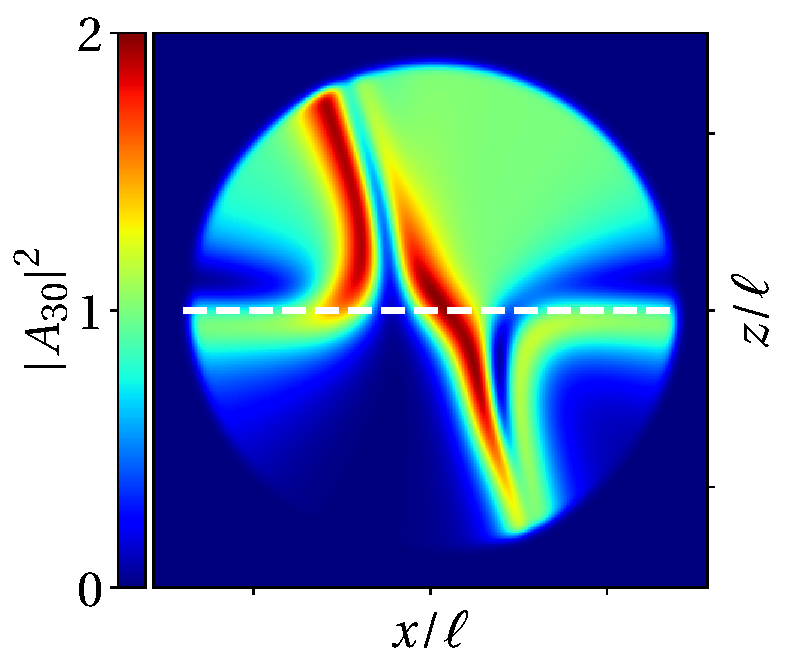
\includegraphics[width=0.33\textwidth]
            {gfx/ch-spin2/UN-BN_SQV-SQV_longitudinal_a30.pdf}};

        \node at (4.8, 2.2) {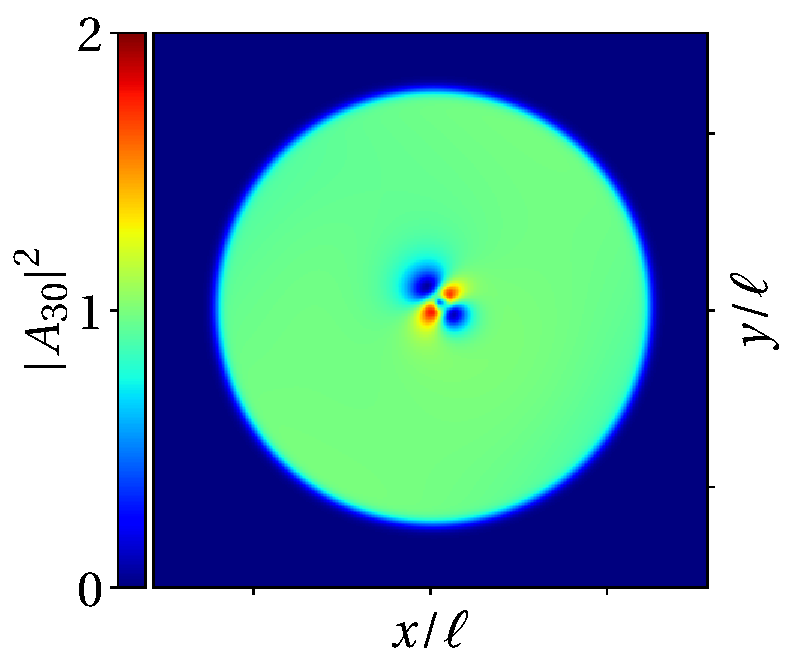
\includegraphics[width=0.33\textwidth]
            {gfx/ch-spin2/UN-BN_SQV-SQV_a30_UN.pdf}};

        \node at (4.8, -2.7) {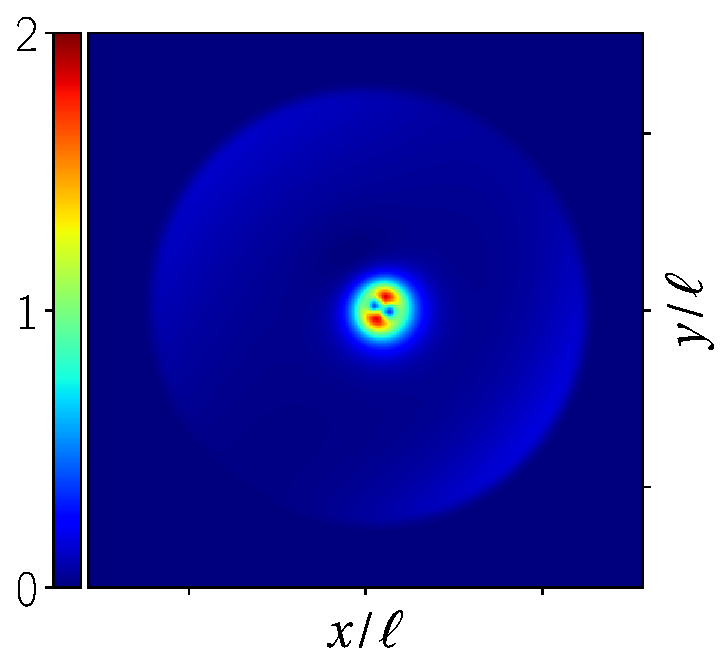
\includegraphics[width=0.33\textwidth]
            {gfx/ch-spin2/UN-BN_SQV-SQV_a30_BN.pdf}};

        \node at (10, 2.35) {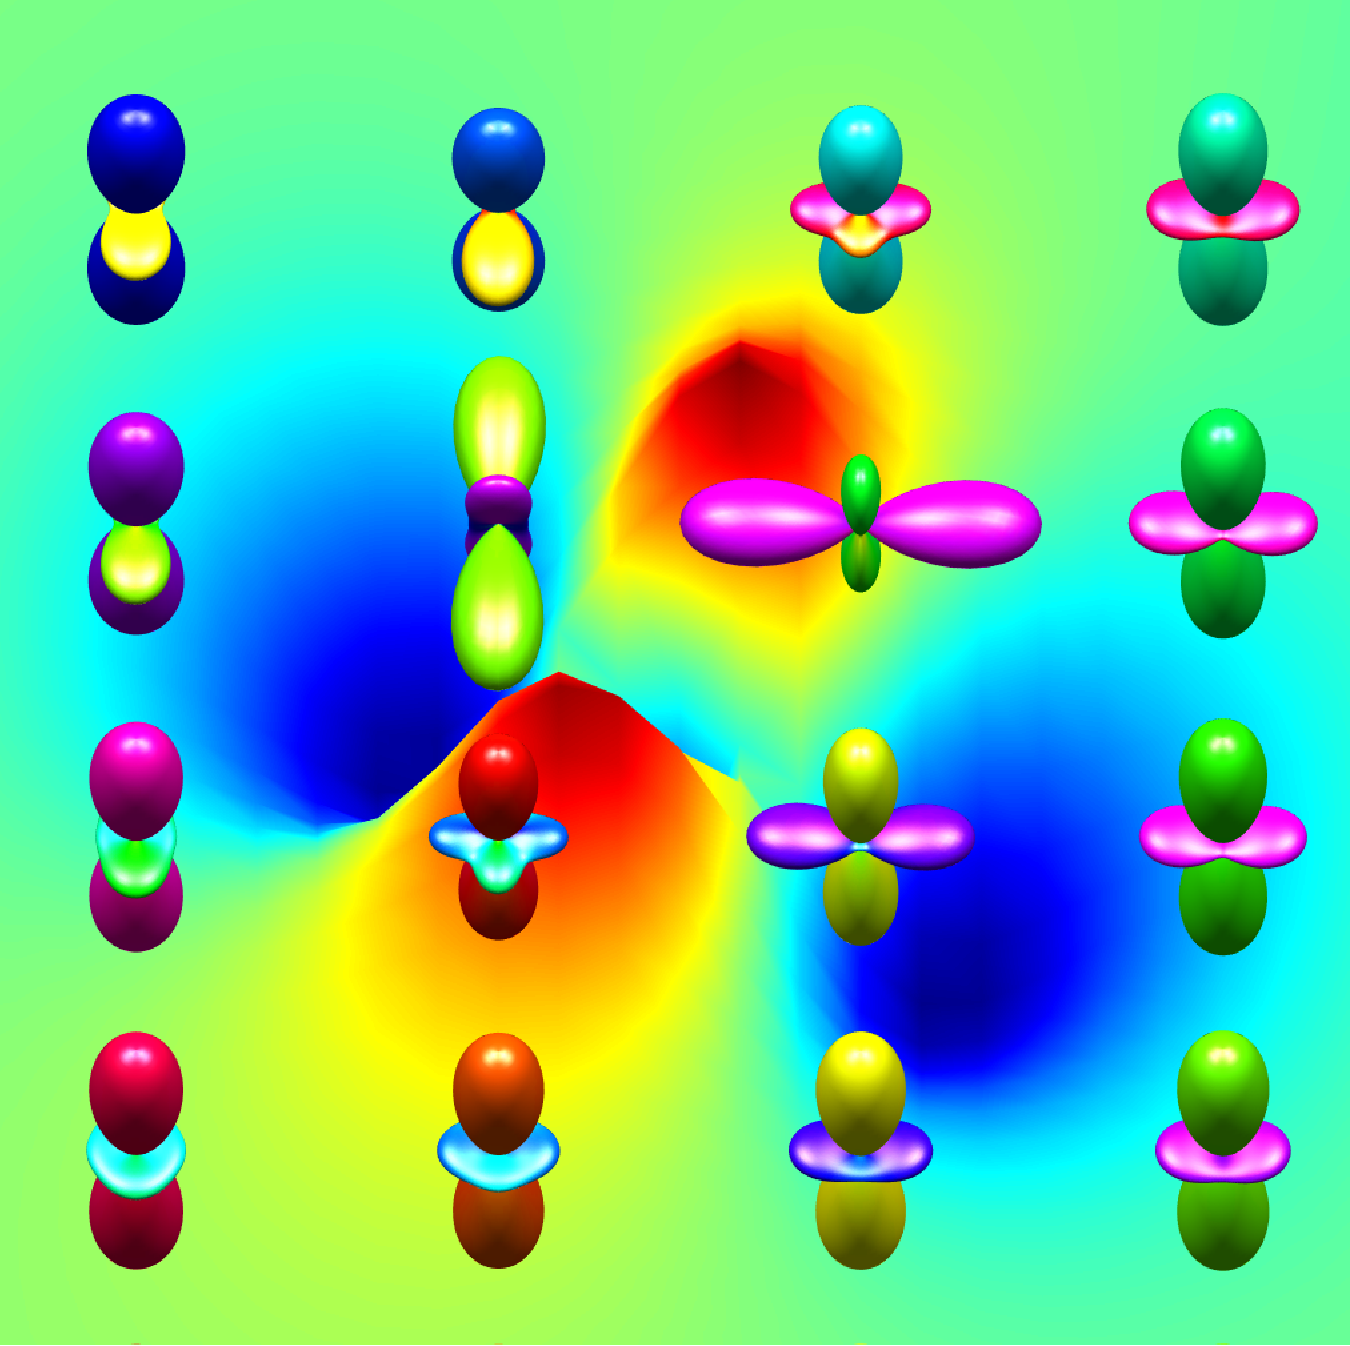
\includegraphics[width=0.26\textwidth]
            {gfx/ch-spin2/UN-BN_SQV-SQV_singletTrio_UN.png}};
        \node[rectangle, draw=black, minimum width=0.55cm,
            minimum height=0.55cm]
        (UN_small_rec) at (5.05, 2.45) {};
        \node[rectangle, draw=black, minimum width=3.8cm,
            minimum height=3.8cm]
        (UN_big_rec) at (10, 2.33) {};
        \draw[-, dashed] (UN_big_rec.north west) -- (UN_small_rec.north west){};
        \draw[-, dashed] (UN_big_rec.south west) -- (UN_small_rec.south west){};

        \node at (10, -2.58) {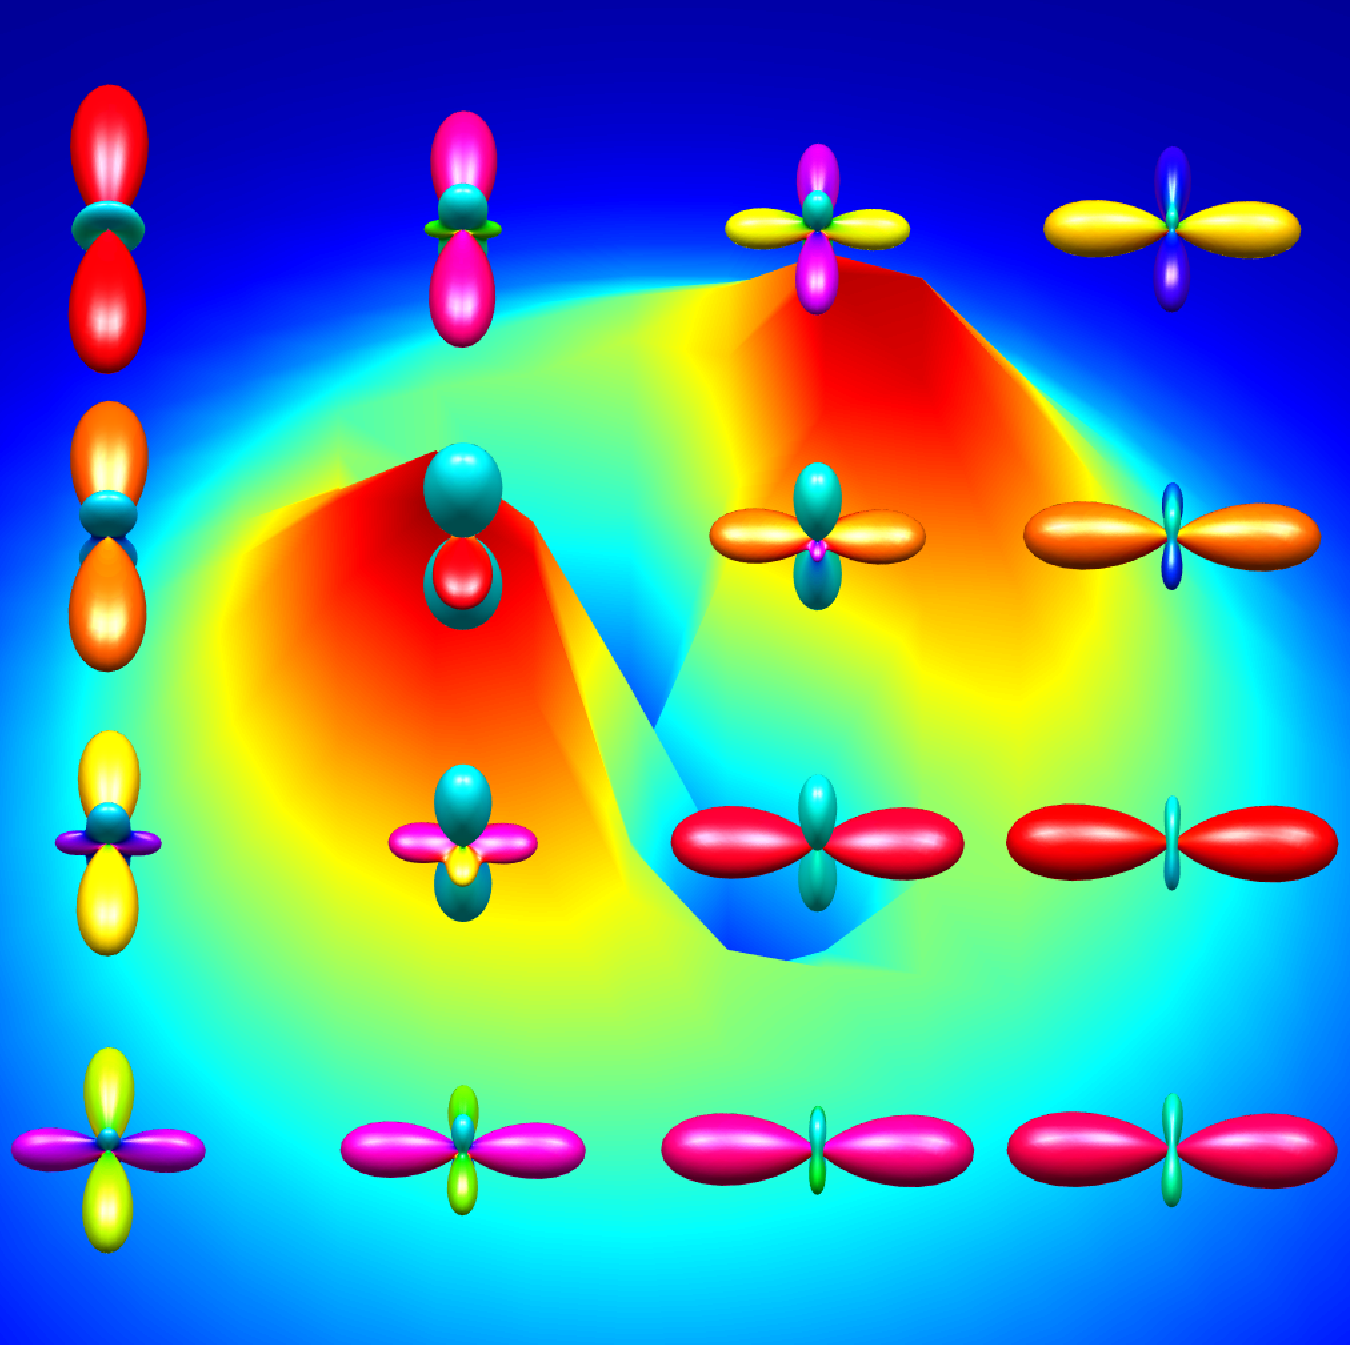
\includegraphics[width=0.26\textwidth]
            {gfx/ch-spin2/UN-BN_SQV-SQV_singletTrio_BN.png}};
        \node[rectangle, draw=black, minimum width=0.55cm,
            minimum height=0.55cm]
        (BN_small_rec) at (5.1, -2.52) {};
        \node[rectangle, draw=black, minimum width=3.8cm,
            minimum height=3.8cm]
        (BN_big_rec) at (10, -2.57) {};
        \draw[-, dashed] (BN_big_rec.north west) -- (BN_small_rec.north west){};
        \draw[-, dashed] (BN_big_rec.south west) -- (BN_small_rec.south west){};

        \node at (0, -2.5) {(a)};
        \node at (5, -0.3) {(b)};
        \node at (5, -5.2) {(c)};
        \node at (10, -0.3) {(d)};
        \node at (10, -5.2) {(e)};
    \end{tikzpicture}
    \caption[Dynamics of a singly quantised vortex connection across a uniaxial
        nematic to biaxial nematic interface]
    {\label{fig: UN-BN-SQV-SQV-singlets}Spin singlet-trio amplitude for
        the UN-BN SQV-SQV connection given in Eq.~\eqref{eq: UN-BN-SQV-SQV} at
        \(\bar{t} = 300\).
        (a): Longitudinal cut showing the spatial separation of the two vortex
        lines.
        (b) and (c): Transverse cut on the UN (\(z/\ell = 3.125\)) and BN
        (\(z/\ell = -3.125\)) sides, respectively, showing the SQVs and their
        composite core structure.
        (d) and (e): Magnified transverse cuts with an overlay of the spherical
        harmonics, showing the non-trivial change of symmetry of the order
        parameter within the vortex cores.}
\end{figure}
In the UN case, the initially empty core fills with atoms occupying both the
cyclic and BN phases, generating a topological interface within the core itself.
This likely arises due to the differing phases factors between the spinor
components, as seen in Fig.~\ref{fig: UN-BN-duo-trio}.
The SQV on the BN side undergoes a similar filling of the empty vortex core,
filling with atoms in the UN, BN and cyclic phases, also generating an interface
within the core.
The development of this composite core structure signifies the start of a
splitting process, whereby the SQV is expected to split into two HQVs
[\textcolor{red}{refs?}].
Since our system has no rotation of the trapping potential to stabilise the
vortices, the timescales considered here reveal that both vortices eventually
leave the condensate cloud.
Additionally, the SQV on the BN side of the interface is observed to leave the
condensate before the splitting into two HQVs has occurred.

We next investigate a vortex connection that terminates on the interface.
We start with the initial state in Eq.~\eqref{eq: UN-BN-vf-sqv}, which contains
no phase winding in the middle component.
The result is a SQV in the BN phase that smoothly connects to a vortex-free
state in the UN phase.
The resulting spin magnitude and singlet-trio amplitude after purely
imaginary-time relaxation are plotted in Fig.~\ref{fig: UN-BN-VF-SQV}.
\begin{figure}
    \centering
    \begin{subfigure}{0.45\textwidth}
        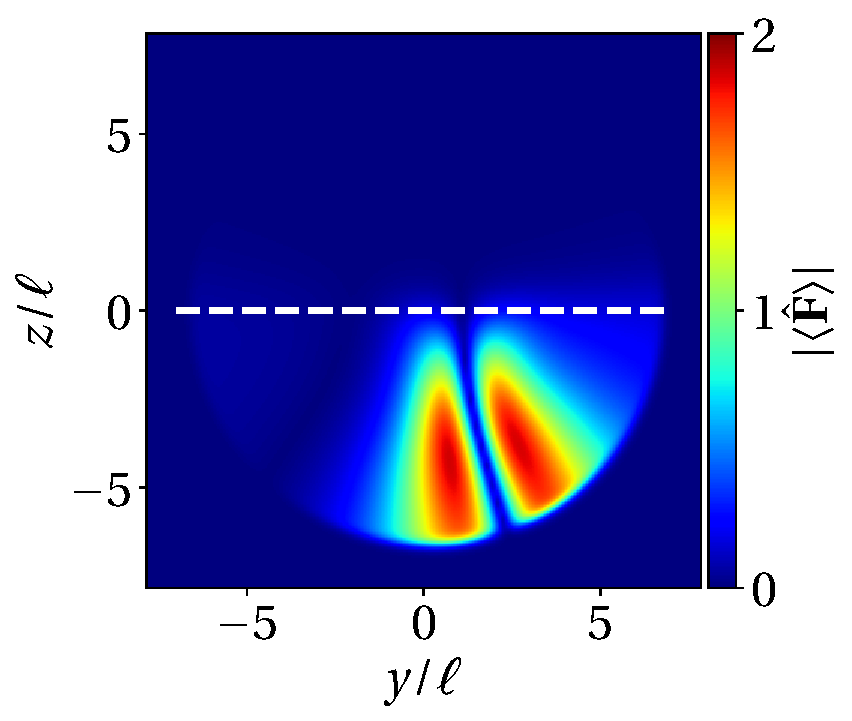
\includegraphics[width=\textwidth]
        {gfx/ch-spin2/UN-BN_VF-SQV_spin_mag.pdf}
        \caption{}
    \end{subfigure}
    \begin{subfigure}{0.45\textwidth}
        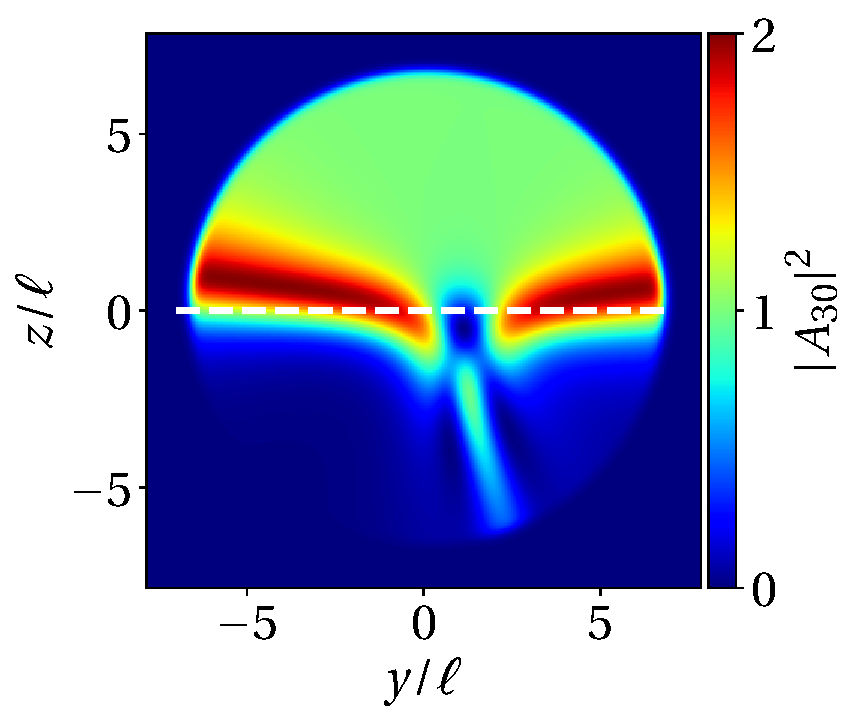
\includegraphics[width=\textwidth]{gfx/ch-spin2/UN-BN_VF-SQV_a30.pdf}
        \caption{}
    \end{subfigure}
    \caption[Dynamics of a singly quantised vortex to vortex-free connection in
    a uniaxial nematic to biaxial nematic interface]
    {\label{fig: UN-BN-VF-SQV} Vortex-free to SQV connection defined
    by Eq.~\eqref{eq: UN-BN-SQV-SQV} with \(\beta=0\) and no winding in the
    middle component.
    (a): Spin magnitude at \(\bar{t}=5\). The HQV cores are identified where
    \(\spinmag = 2\).
    (b): Spin-singlet trio amplitude at \(\bar{t} = 5\). A cyclic region is
    revealed where \(|A_{30}|^2 = 2\), which arises due to phase differences
    (see Fig~\ref{fig: UN-BN-duo-trio}).}
\end{figure}
The dynamics of this connection closely resembles what the later dynamics of the
BN side of the SQV-SQV connection would look like, provided that the vortices
were stabilised against leaving the condensate.
We see that the initial SQV on the BN side has undergone a splitting process
into two HQVs, each of which can be seen to terminate at the interface.
The cores of the HQVs are easily identified from the
\(\spinmag = 2\) regions.
Similar splitting of an SQV into HQVs has been observed in the polar phase of
spin-1 condensates~\cite{Seo2015, Xiao2021}.
For the timescales considered, the resulting HQVs remain stable against
leaving the condensate.
Additionally, we see the clear presence of the cyclic phase emerging at the
interface \(z / \ell \sim 0\), arising due to the phase difference between
the spinor components (see Fig.~\ref{fig: UN-BN-duo-trio}).

\subsection{Cyclic to ferromagnetic interface}
We numerically investigate vortex connections across a topological interface
between the cyclic and FM-2 phases, given by
Eq.~\eqref{eq: C-FM-interpolating-spinor}.
Since our numerical simulations use parameters that predict a nematic ground
state, we introduce a spatially-dependent \(c_1\) term such that \(c0/c_1=90.7\)
on the cyclic side but \(c_0/c_1=-90.7\) on the FM side, effectively changing
the sign of the \(c_1\) term.
\textcolor{red}{Are there experimental papers to cite here that mention the
manipulation of scattering lengths to achieve this?}
Now, in the FM region, the parameters ensure that the FM region remains stable.
Despite the cyclic state not being the predicted ground state, the interface
is observed to remain stable for the timescales considered in our simulations.

We firstly investigate the connection of a third vortex in the cyclic phase
connecting to a singular SQV in the FM-2 phase using
Eq.~\eqref{eq: C-FM-third-sqv} as the initial state.
This initial state is then propagated using a short imaginary-time evolution to
imprint the vortex cores and, once the core is imprinted, we switch to
complex-time simulations using a damping coefficient of \(\nu=10^{-2}\).
The resulting spin magnitude and spin-singlet duo amplitude for this interface
after time \(\bar{t} = 5\) are plotted in Fig.~\ref{fig: C-FM-third-SQV}.
\begin{figure}
    \centering
    \begin{tikzpicture}

        \node[inner sep=0pt] (plot1) at (-5,0)
        {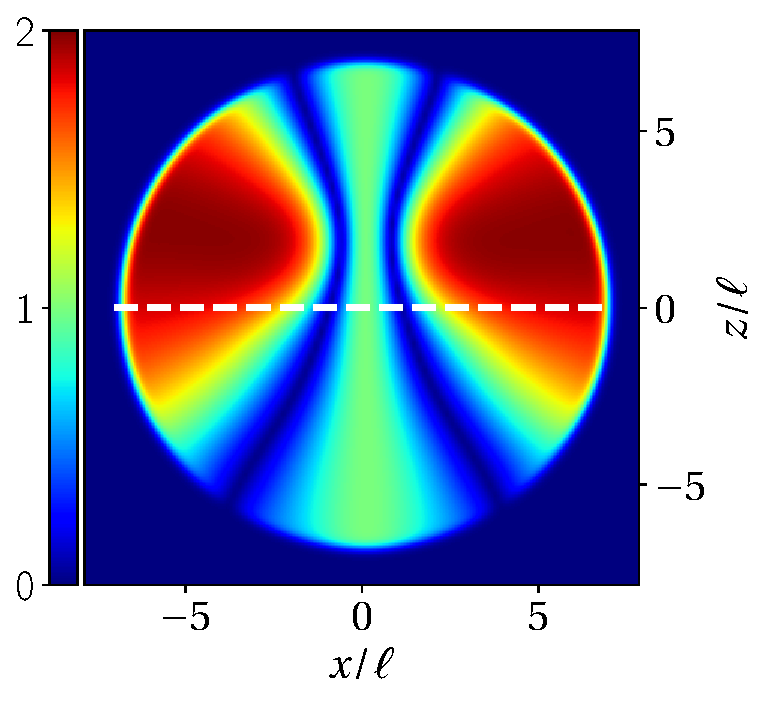
\includegraphics[width=0.33\textwidth]
            {gfx/ch-spin2/C-FM=2_third-SQV_spin_mag.pdf}};
        \node[inner sep=0pt] (plot2) at (-0.6, 0.25)
        {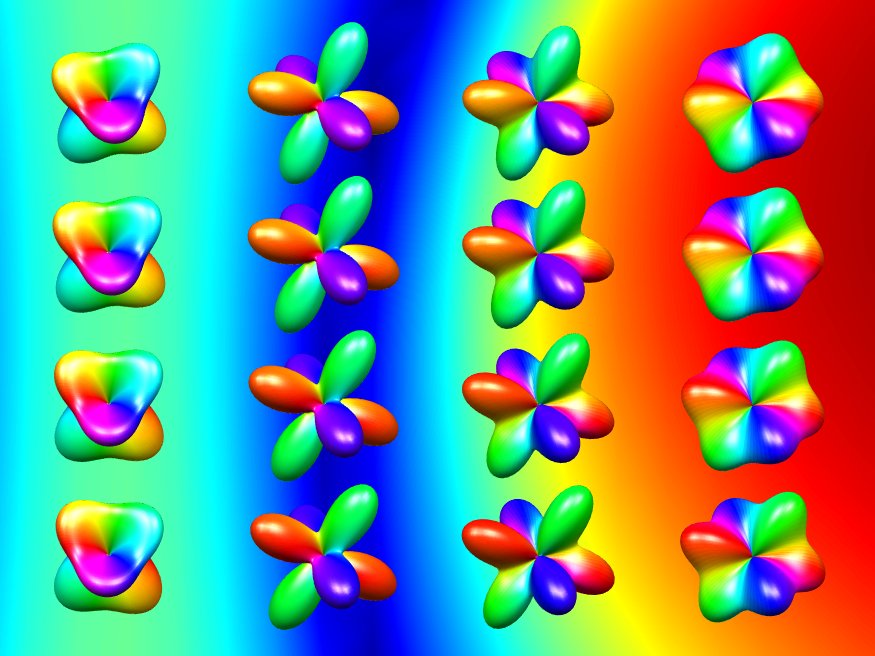
\includegraphics[width=0.25\textwidth, height=0.25\textwidth]
            {gfx/ch-spin2/C-FM=2_third-SQV_spinMag_spherical.pdf}};
        \node[rectangle, draw=black, minimum width=0.5cm, minimum height=0.5cm]
        (rec) at (-4.75, 0.75) {};
        \draw[-, dashed] (rec.north west) -- (plot2.north west) {};
        \draw[-, dashed] (rec.south west) -- (plot2.south west) {};

        \draw[-, thick] (plot2.south east) -- (plot2.north east) {};
        \draw[-, thick] (plot2.south east) -- (plot2.south west) {};
        \draw[-, thick] (plot2.south west) -- (plot2.north west) {};
        \draw[-, thick] (plot2.north west) -- (plot2.north east) {};

        \node[inner sep=0pt] (plot0) at (3.8,0)
        {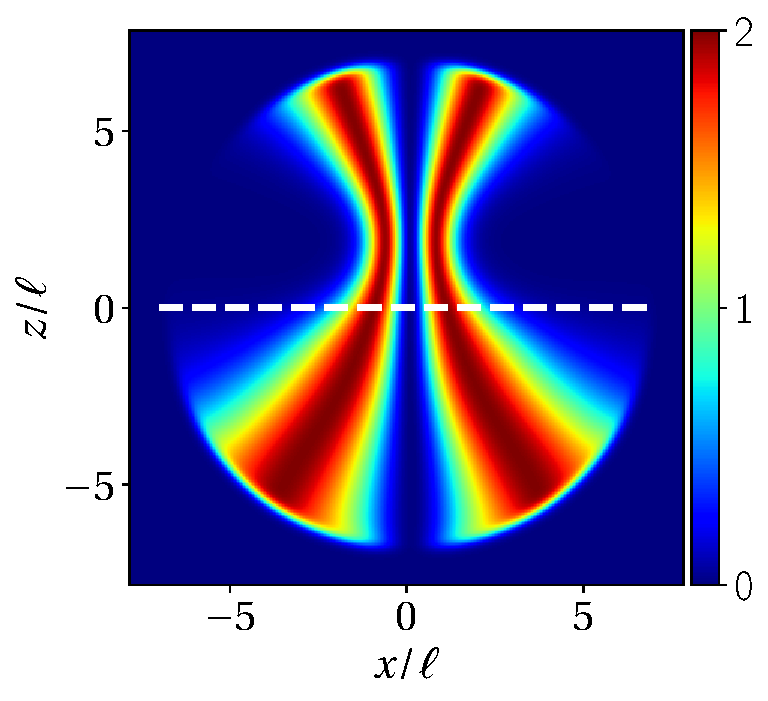
\includegraphics[width=0.33\textwidth]
            {gfx/ch-spin2/C-FM=2_third-SQV_singlet_trio.pdf}};

        \node[inner sep=0pt] (plot3) at (-0.7, -5) {
            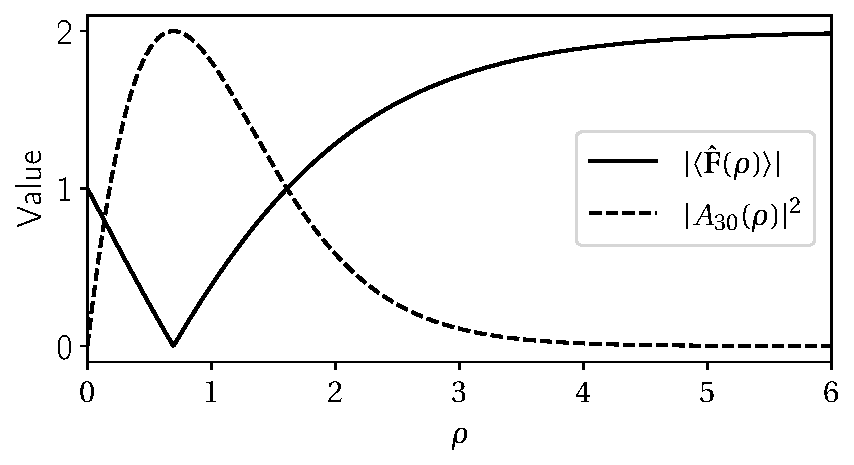
\includegraphics[width=0.5\textwidth]
                {gfx/ch-spin2/spin_singlet_radius_analytical.pdf}
        };

        % Labels
        \node at (-5.15, -2.5) {(a)};
        \node at (-0.5, -2.5) {(b)};
        \node at (3.95, -2.5) {(c)};
        \node at (-0.5, -7.5) {(d)};
    \end{tikzpicture}
    \caption[Dynamics of a one-third vortex to singly quantised vortex
    connection in a cyclic to ferromagnetic interface]
    {\label{fig: C-FM-third-SQV}Third vortex to SQV connection in an
    interface between the cyclic and FM-2 phases given by
    Eq.~\eqref{eq: C-FM-third-sqv} at \(\bar{t} = 50\).
    (a): Longitudinal cut of \(\spinmag \) at \(y/\ell=0\).
    The third vortex on the cyclic side (\(z/\ell < 0\)) is evident from the
    \(\spinmag = 1\) core which extends throughout the FM region.
    (b): Zoomed transverse cut of \(\spinmag \) inside the core in the FM
    region.
    Overlaid are the spherical harmonics showing the non-trivial change
    of order parameter symmetry inside the core.
    (c): Longitudinal cut of \(|A_{30}|^2\) at \(y/\ell=0\).
    Cyclic regions are identified from \(|A_{30}|^2=2\).
    (d) Analytically calculated values of \(\spinmag \) and \(|A_{30}|^2\)
    using the interpolating spinor in Eq.~\eqref{eq: C-FM-third-sqv} with the
    choice of \(\eta(\rho) = 3\tanh(\rho/3)\).}
\end{figure}
Here, \(\spinmag \) reveals non-trivial core structures emerging.
Clearly one can see the third vortex on the cyclic side of the interface
(\(z/\ell < 0\)) evidenced by the \(\spinmag = 1\) core.
However, unlike the previous case where the vortices spatially separated, this
\(\spinmag = 1\) region then extends throughout the longitudinal extent of the
condensate, and penetrates into the FM region, revealing that the initial SQV of
the FM phase has developed a composite core structure.
This composite core structure is separated into three distinct parts:
Inside is the \(\spinmag = 1\) region, which is then encased in a cyclic shell
as seen from the \(|A_{30}|^2=2\) regions in Fig.~\ref{fig: C-FM-third-SQV}c.
Then, far away from the vortex core, the system smoothly interpolates back to
a \(\spinmag = 2\) region in the bulk of the condensate.
The spherical harmonics of the internal core structure plotted in
Fig.~\ref{fig: C-FM-third-SQV}b reveal the non-trivial change of order parameter
symmetry within the composite core.

One can use the general spinor in Eq.~\eqref{eq: C-FM-third-sqv} to
analytically examine the vortex core structures when \(\eta \) is a
function of the transverse radius \(\rho = \sqrt{x^2 + y^2}\).
The states can be described by choosing an appropriate function for
\(\eta(\rho)\) that interpolates between all three phases.
We choose \(\eta(\rho) = 3\tanh(\rho/2) - 1\) which becomes \(\eta=-1\) at
\(\rho=0\), \(\eta=0\) and hence cyclic at \(\rho=\tanh^{-1}(1/3)\), and
finally \(\eta=2\) at large \(\rho \).
The resulting spin magnitude and singlet-trio amplitude using the above
substitution in Eq.~\eqref{eq: C-FM-third-sqv} are plotted in
Fig.~\ref{fig: C-FM-third-SQV}d.
We see that the analytically calculated values of \(\spinmag \) and
\(|A_{30}|^2\) mirror those observed in the numerics.

Instead of considering only singular vortices, we can also investigate the
coreless vortex connection given in Eq.~\eqref{eq: C-FM-coreless-general}.
We choose this as the initial state, with
\(\beta = \pi\left(1 + \tanh(\rho-1)\right)/2\) to model the required
monotonically increasing function.
Here we focus only on the cyclic to FM-2 limit, but equivalently the cyclic to
FM-1 limit can be chosen by an appropriate choice of \(p\) and \(q\) that
interpolates \(\eta \) between \(-1\) and \(0\).
We perform purely imaginary-time simulations to simulate energy relaxation.
\begin{figure}
    \centering
    \begin{tikzpicture}
        % DQV
        \node[inner sep=0pt] (initial_dqv) at (0.4, 0)
        {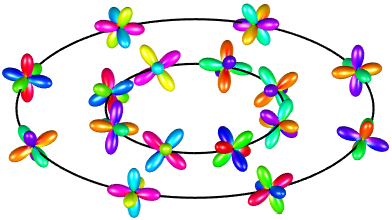
\includegraphics[width=0.3\textwidth]
            {gfx/ch-spin2/C-FM=2_coreless_cyclic_init_spherical.pdf}};
        \node[cylinder, draw, fill=black, opacity=0.5, minimum height=3cm,
            rotate=90] (c_dqv) at (0.4, 0) {};

        % Colour bar
        \node[rotate=90] at (-2.15, 0.2)
        {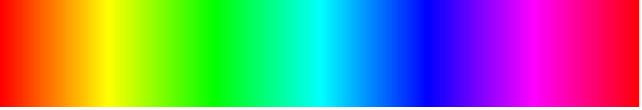
\includegraphics[width=0.15\textwidth, height=0.015\textheight]
            {gfx/colourbars/hsv_colourbar.pdf}};
        \node[rotate=90] at (-2.15, -1.8) {Arg(\(Z\)) = 0};
        \node[rotate=90] at (-2.15, 1.7) {\(2\pi \)};

        % Spin mag
        \node[inner sep=0pt] (spinmag_dqv) at (5, 0)
        {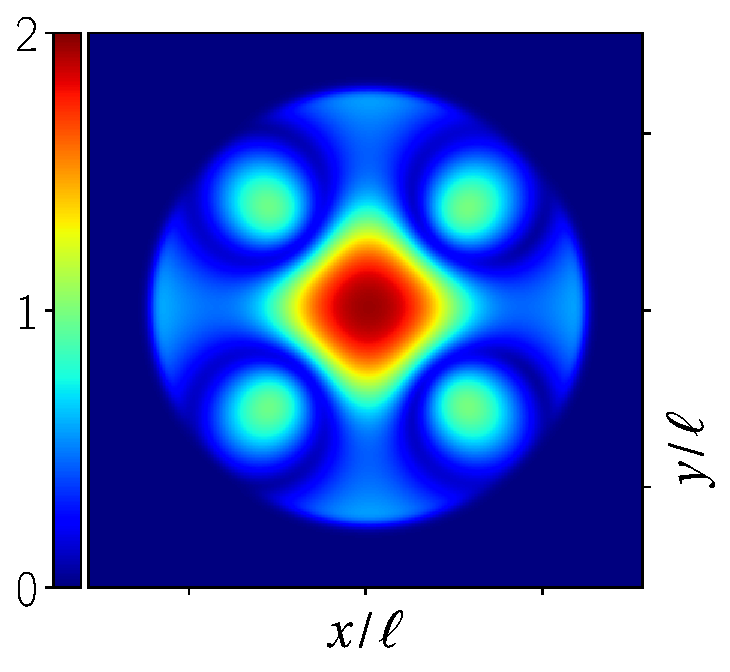
\includegraphics[width=0.3\textwidth]
            {gfx/ch-spin2/C-FM=2_coreless_cyclic_spin_mag.pdf}};

        % Third spherical
        \node[inner sep=0pt] (third_spherical) at (10, 1.5)
        {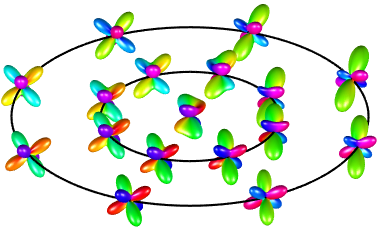
\includegraphics[width=0.3\textwidth]
            {gfx/ch-spin2/C-FM=2_coreless_cyclic_third_spherical.pdf}};
        \node[cylinder, draw, fill=green, opacity=0.5, minimum height=2.8cm,
            rotate=90] (c_third) at (10, 1.5) {};
        \node[rectangle, draw, minimum width=0.3cm, minimum height=0.3cm,
            dashed, green]
        (third_small_rec) at (5.28, 0.62) {};
        \node[rectangle, draw, minimum width=4.4cm, minimum height=2.9cm,
            green] (third_big_rec) at (10, 1.6) {};
        \draw[-, dashed, green]
        (third_big_rec.north west) -- (third_small_rec.north west) {};
        \draw[-, dashed, green]
        (third_big_rec.south west) -- (third_small_rec.south east) {};

        % Two-third spherical
        \node[inner sep=0pt] (third_spherical) at (10, -1.5)
        {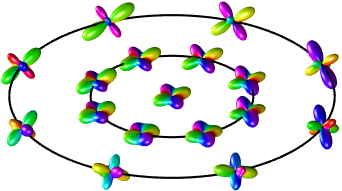
\includegraphics[width=0.3\textwidth]
            {gfx/ch-spin2/C-FM=2_coreless_cyclic_2third_spherical.pdf}};
        \node[cylinder, draw, fill=red, opacity=0.5, minimum height=2.8cm,
            rotate=90] (c_2third) at (10, -1.5) {};
        \node[rectangle, draw, dashed, minimum width=0.7cm,
            minimum height=0.7cm, rotate=45, opacity=0.5, red]
        (2third_small_rec) at (4.8, 0.15) {};
        \node[rectangle, draw, minimum width=4.4cm, minimum height=2.9cm,
            red] (2third_big_rec) at (10, -1.4) {};
        \draw[-, dashed, red]
        (2third_big_rec.north west) -- (2third_small_rec.south east) {};
        \draw[-, dashed, red]
        (2third_big_rec.south west) -- (2third_small_rec.south west) {};

        % Labels
        \node at (0.4, -2.3) {(a)};
        \node at (5, -2.3) {(b)};
        \node at (8.2, 2.7) {(c)};
        \node at (8.2, -0.3) {(d)};
    \end{tikzpicture}
    \caption[Dynamics of the doubly quantised vortex connection in a cyclic to a
        ferromagnetic interface]
    {\label{fig: C-FM-coreless-cyclic}Schematic representation of the
        splitting process occurring on the cyclic side of the interface
        (\(z/\ell < 0\)) given by the state in
        Eq.~\eqref{eq: C-FM-coreless-general}.
        (a): Spherical harmonic representation of the initial doubly quantised
        vortex line. By traversing a point about the vortex line, the condensate
        phase is seen to wind by \(4\pi \).
        (b) Transverse cut of \(\spinmag \) at \(z/\ell \approx -3\) after
        imaginary-time evolution at \(\bar{t} = 1.5\) showing the splitting of
        the initial doubly quantised vortex into fractional vortices.
        The one-third and two-third vortices are clearly identified from the
        \(\spinmag = 1\) and \(\spinmag = 2\) regions, respectively.
        (c) and (d): Spherical harmonic representations about the one-third and
        two-third vortices, respectively.
        The spherical harmonics shows the non-trivial change of the order
        parameter symmetry as we move away from the vortex cores.}
\end{figure}
We start by discussing the dynamics of the doubly quantised vortex on the cyclic
side of the interface, shown in Fig.~\ref{fig: C-FM-coreless-cyclic}.
As expected for a doubly quantised vortex line, it very rapidly undergoes a
splitting process.
In this case, it splits into four one-third vortices, evidenced by the
\(\spinmag = 1\) regions, and a further two-third vortex, evidence by the large
\(\spinmag = 2\) region.
The discrepancy of the core size could arise from the different vortices being
set by different healing lengths.
Analysis of the spherical harmonics in Fig.~\ref{fig: C-FM-coreless-cyclic}c,d
shows the non-trivial order parameter symmetry both within and outside the
vortex cores.
By following the spherical harmonics about the vortex cores, the condensate
phase changes by \(2\pi/3\) and \(4\pi/3\) confirming that these structures are
one-third and two-third vortices.
Due to the energy relaxation, the one-third vortices quickly leave the
condensate.
However, the two-third vortex is first observed to undergo a further splitting
process in which it splits into two one-third vortices, which then proceed to
exit the condensate cloud.

The initial coreless vortex on the FM side of the interface also undergoes a
complex splitting process, shown in Fig.~\ref{fig: C-FM-coreless-FM}.
\begin{figure}
    \centering
    \begin{tikzpicture}
        % DQV
        \node[inner sep=0pt] (initial_coreless) at (0.4, 0)
        {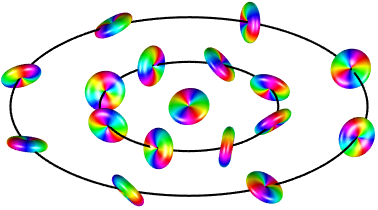
\includegraphics[width=0.3\textwidth]
            {gfx/ch-spin2/C-FM=2_coreless_FM_init_spherical.pdf}};

        % Colour bar
        \node[rotate=90] at (-2.15, 0.2)
        {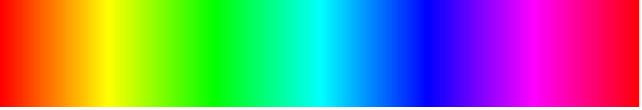
\includegraphics[width=0.15\textwidth, height=0.015\textheight]
            {gfx/colourbars/hsv_colourbar.pdf}};
        \node[rotate=90] at (-2.15, -1.8) {Arg(\(Z\)) = 0};
        \node[rotate=90] at (-2.15, 1.7) {\(2\pi \)};

        % Spin mag
        \node[inner sep=0pt] (spinmag_coreless) at (5, 0)
        {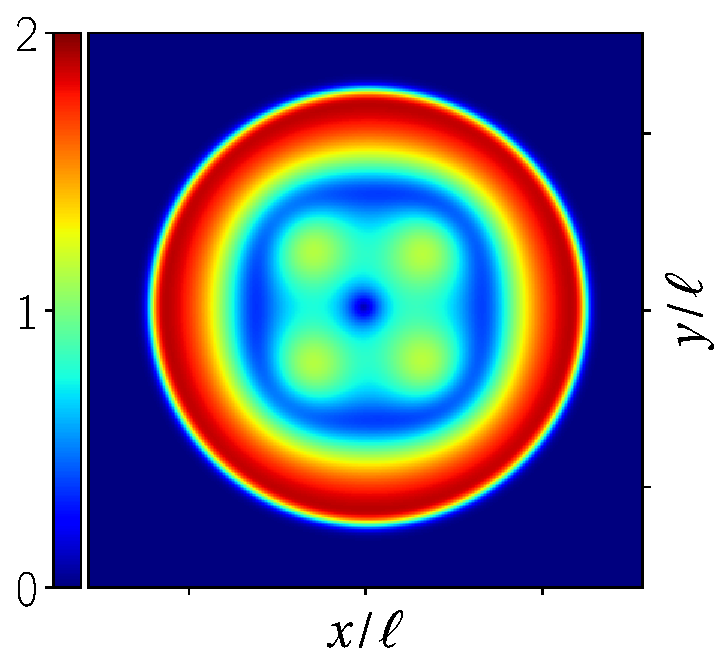
\includegraphics[width=0.3\textwidth]
            {gfx/ch-spin2/C-FM=2_coreless_FM_spin_mag.pdf}};

        % After splitting
        \node[inner sep=0pt] (initial_dqv) at (10, 0)
        {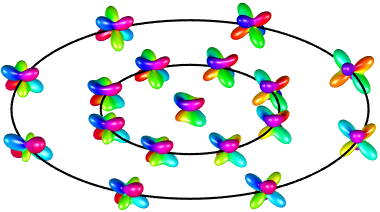
\includegraphics[width=0.3\textwidth]
            {gfx/ch-spin2/C-FM=2_coreless_FM_after_spherical.pdf}};

        \node[rectangle, draw, minimum width=0.5cm, minimum height=0.5cm]
        (small_rec) at (5.1, -0.1) {};
        \node[rectangle, draw, minimum width=4.4cm, minimum height=2.3cm]
        (big_rec) at (10, 0) {};
        \draw[-, dashed] (big_rec.north west) -- (small_rec.north east) {};
        \draw[-, dashed] (big_rec.south west) -- (small_rec.south east) {};
    \end{tikzpicture}
    \caption[Dynamics of the coreless vortex in a cyclic to ferromagnetic
        interface]
    {\label{fig: C-FM-coreless-FM}Schematic representation of the
        splitting process occurring on the FM side of the interface
        (\(z/\ell > 0\)) of the state in Eq.~\eqref{eq: C-FM-coreless-general}.
        (a): Spherical harmonic representation of the initial coreless vortex,
        defined explicitly in Eq.~\eqref{eq: C-FM-coreless-FM-limits}.
        (b) Transverse cut of \(\spinmag \) at \(z/\ell \approx 3\) after
        complex-time evolution at \(\bar{t} = 1.5\).
        The singular vortex structures can be seen from the
        \(\spinmag \approx 1\) cores.
        (c): Spherical harmonic representation of the internal structure of
        the singular vortex, showing the non-trivial symmetry within the core.}
\end{figure}
The coreless structure is observed to split into four singular vortices,
observed from transverse cuts of \(\spinmag \).
Analysis of the spherical harmonics reveal the non-trivial symmetry within
the singular vortex cores.
As in the case on the cyclic side, these vortices rapidly leave the condensate
due to the energy relaxation.
On both sides of the interface the vortex structures are observed to terminate
at the interface itself, and do not connect in a way that is observed in the
SQV to one-third vortex connection (see Fig.~\ref{fig: C-FM-third-SQV}).
